% !Mode:: "TeX:UTF-8"
\documentclass[doctor,openright,twoside,color]{buaathesis}
\begin{document}

% 用户信息
% !Mode:: "TeX:UTF-8"

% 学院中英文名,中文不需要“学院”二字
% 院系英文名可参见
% http://ev.buaa.edu.cn/education/index.php?page=department
\school
{航空科学与工程}{School of Aeronautic Science and Engineering}

% 专业中英文名,中文不需要“专业”二字
\major
{飞行器设计}{Aircraft Design}

% 论文中英文标题
\thesistitle
{长标题}
{副标题}
{English title}
{English sub title}

% 作者中英文名
\thesisauthor
{裴为诚}{PEI Weicheng}

% 导师中英文名
\teacher
{李书}{LI Shu}

% 中图分类号,可在 http://www.ztflh.com/ 查询
\category{V211.52}% 直升飞机、旋翼机空气动力学

% 本科生为毕设开始时间;研究生为学习开始时间
\thesisbegin{2014}{09}{01}

% 本科生为毕设结束时间;研究生为学习结束时间
\thesisend{2018}{06}{01}

% 毕设答辩时间
\defense{2018}{06}{01}

% 中文摘要关键字
\ckeyword{直升机,空气动力学,旋翼尾迹,舰船空气尾流,气动干扰}

% 英文摘要关键字
\ekeyword{Helicopter, Aerodynamics, Rotor Wake, Ship Airwake, Aerodynamic Interaction}

% master_info.tex
% !Mode:: "TeX:UTF-8"

% 研究方向
\direction{旋翼空气动力学、直升机空气动力学}

% 教师职称中英文
\teacherdegree{教授}{Prof.}

% 保密等级
\mibao{公开}

% 论文编号,由10006+学号组成
\thesisID{10006BY1405156}

% 论文提交时间
\commit{2018}{06}{01}

% 学位授予日期
\award{2018}{06}{30}



% 中英封面、提名页、授权书
%\maketitle
% 前言页眉页脚样式
\pagestyle{frontmatter}
% 摘要
% !Mode:: "TeX:UTF-8"
\begin{cabstract}
直升机特有的垂直起降和悬停飞行能力,特别适合于在海上平台执行作业任务。
在所有与舰载直升机相关的力学问题中,空气动力学是最核心、最关键的问题。
对舰载直升机而言,空气动力学的研究内容主要包含两部分:
一是所有旋翼飞行器所共有的一般性问题,二是舰船所带来的特殊问题。

旋翼流场由桨尖涡主导,具有非定常、非线性的特点,复杂程度高于固定翼流场。
对旋翼空气动力学的研究主要分为实验和数值计算两大类。
实验研究经历了从定性到定量、从宏观力学参数测量到全流场流动细节捕捉的发展过程。
数值计算方面,相继发展出了入流模型、涡线尾迹模型、黏性涡粒子模型、基于欧拉观点的涡量输运方程模型、雷诺平均Navier-Stokes方程模型等分析方法。
由于旋翼空气动力学本身的复杂性和现有研究手段的局限性,该领域目前仍是空气动力学研究的热点和难点。

海面自由来流经过舰船表面结构,形成紊乱的空气尾流,与旋翼尾迹的相互作用,形成舰载直升机所特有的空气动力学问题。
舰载直升机处于舰面起降过程中时,海面和舰面会对旋翼产生“地”面效应,这也是海面、舰面与旋翼之间复杂气动干扰的一种形式。
把握上述气动干扰的规律,是舰载直升机空气动力学的主要研究内容。
与旋翼空气动力学类似,该领域的研究方法也分为实验和计算两大类。

本文对舰载直升机空气动力学的国内外研究现状进行了综述,并对与舰载直升机相关的一些应用问题作了简要介绍。
\end{cabstract}
%
\begin{eabstract}
Helicopter is particularly suitable for offshore platforms, for its unique ability of vertical taking off and landing and hovering.
Among all the problems of mechanics on a ship borne helicopter, aerodynamics is the most important and key one.
It mainly contains two kinds of problems, one is about the common problems of rotorcraft aerodynamics, the other is the specific issues brought by the ship.

The flow field of a rotor is dominated by the tip vortices.
It is much more sophisticated than that of a fixed wing, since it is highly unsteady and nonlinear.
There are two major categories of research approaches: experiment and numerical calculation.
Experimental studies have experienced great development from qualitative to quantitative, from measuring macro mechanical parameters to capturing details of the entire flow field.
In the aspect of numerical calculation studies, different kinds of calculation models have been developed, such as rotor inflow models, vortex line wake models, the viscous vortex particle model, 
the Eulerian vorticity transport equation model, the Reynolds averaged Navier Stokes equation model, etc..
Due to the complexity of the rotor aerodynamics and the limitations of existing research methods, this field will continue to be a hot and difficult spot in the school of aerodynamics.

As free winds pass through the building structures on the deck of a ship, chaotic ship airwakes are formed at the same time.
When a helicopter is performing a taking off or landing task, there are strong and complex interactions between the wake of its rotor(s) and the ship airwakes.
Ground effects can also be experienced by the rotor(s) during this task, because of the existence of the sea surface and the ship deck.
It is the most important task for ship borne helicopter aerodynamics to understand such sea-ship-helicopter aerodynamic interactions. 
The research methods in this field, like those in rotor aerodynamics, is also divided into two categories: experimental and computational.

In this paper, the research status of rotor aerodynamics and ship borne helicopter aerodynamics, both in China and abroad, has been reviewed.
Some problems related to the application of the ship borne helicopters are briefly introduced.
\end{eabstract}
  
% 目录、插图目录、表格目录
\tableofcontents
\listoffigures
%\listoftables
% 符号表
% !Mode:: "TeX:UTF-8"
\begin{denotation}
%%%%%%%%%%%%%%%%%%%
\item[$Re$] 雷诺数(Reynolds number)
\item[$M$] 马赫数(Mach number)
%%%%%%%%%%%%%%%%%%%
\item[AMR] 自适应网格加密(Adaptive Mesh Refinement)
\item[CFD] 计算流体动力学(Computational Fluid Dynamics)
\item[DNS] 直接数值模拟(Direct Numerical Simulations)
\item[FEM] 有限元方法(Finite Element Method)
\item[LDV] 激光多普勒测速技术(Laser Doppler Velocimetry)
\item[LES] 大涡模拟(Large Eddy Simulation)
\item[LTV] 激光断层扫描显示(Laser Tomoscopy Visualizations)
\item[MLPG] 无网格局部彼得罗夫-伽辽金(Meshless Local Petrov-Galerkin)方法
\item[PIV] 粒子成像测速技术(Particle Image Velocimetry)
\item[RANS] 雷诺平均纳维-斯托克斯(Reynolds-Averaged Navier-Stokes)方程
\item[VPM] 黏性涡粒子模型(Vortex Particle Model)
\item[VRS] 涡环状态(Vortex Ring State)
\item[VTM] 涡量输运模型(Vorticity Transport Model)
\item[VTOL] 垂直起降(Vertical Take-Off and Landing)
\end{denotation}


% 正文页码样式
\mainmatter
% 正文页眉页脚样式
\pagestyle{mainmatter}

% 正文
\chapter{概述}

\section{问题背景}
直升机以其特有的垂直起降(Vertical Take-Off and Landing, VTOL)、悬停和低空低速飞行能力,特别适合于在军舰、科考船、海上钻井平台等起降条件和飞行环境较差的平台上执行任务。
舰载直升机能够有效扩大舰船作业半径、丰富海上作业科目、提升应对海上突发情况的能力。
发展舰载直升机对于保障舰船航行安全、维护海洋权益具有重要意义。
世界各海洋大国和航空大国历来重视舰载直升机的发展,相继研制出各种不同构型的舰载直升机(见表\ref{Marine-Helicopter})。
我国海军正处于“近海防御型向近海防御与远海护卫型结合转变”\upcite{PRC2015}的关键时期,发展适合中国国情的舰载直升机,对于实施海洋强国战略具有重要意义。
\begin{longtable}[c]{cccccl}
\caption{国外主要舰载直升机}
\label{Marine-Helicopter}\\\toprule[1pt]
原产国 & 型号 & 别名 & 构型 & 首飞时间 & 服役时间
\\\midrule
美国 & SH-60 & 海鹰(Sea Hawk) & 单主旋翼 & 1979 & 1984-现在  \\
美国 & CH-46 & 海骑士(Sea Knight) & 纵列式 & 1962 & 1964-2004\footnote{美国海军}/2015\footnote{美国海军陆战队}  \\
美国 & V-22 & 鱼鹰(Osprey) & 倾转旋翼 & 1989 & 2007-现在  \\
苏联 & Ка-27/28 & 蜗牛(Helix) & 单主旋翼 & 1973 & 1982-现在  \\
\bottomrule[1pt]
\end{longtable}

在舰载直升机的设计、使用和维护过程中,存在大量亟待解决的科学和工程问题。
其中,既有旋翼飞行器所共有的一般性问题,也有直升机执行海上作业任务所带来的特殊问题。

\section{旋翼飞行器综合分析}
旋翼(Rotor)是以直升机(Helicopter)为代表的旋翼飞行器(Rotorcraft)区别于其他航空飞行器(Aircraft/Aerocraft)的标志性部件。
从力学研究的角度来看,旋翼系统(以及旋翼-机体耦合系统)属于复杂的刚柔耦合多体动力学系统。
与其他复杂系统一样,对旋翼系统(以及旋翼-机体耦合系统)的研究大致可以分为实验和计算两大类。

实验研究,是人们对科学和工程问题所有理性认识的主要来源,也是检验一切物理模型和计算方法合理性的重要依据。
对旋翼飞行器的实验研究,
按实验对象可以分为缩比模型实验、全尺寸样机实验;
按实验环境可以分为风洞实验、试飞实验。
由于代价昂贵,只有少数大型研究机构和企业有能力对旋翼飞行器开展系统的实验研究。

计算研究,是对实验研究的重要补充,有时也被称为数值实验。
它是指从运动学、动力学、空气动力学等学科的基础理论出发,利用计算机,对直升机(特别是旋翼)的力学行为进行分析计算。
相对于模型或样机实验,数值实验拥有巨大的成本优势,这是驱动计算研究不断发展的主要动力。
对于新的设计方案,数值实验能够先于模型或样机实验对其性能指标进行评价,这也是其相对于模型或样机实验所具有的优势。
另外,对于飞行事故等模型或样机实验难以复现的过程,数值实验也是不可替代的研究手段。
可以预见,随着计算机硬件和分析软件水平的不断提高,数值实验将在直升机设计、使用和维护过程中扮演越来越重要的角色。

直升机界于1980年左右提出了“综合分析(Comprehensive Analysis)”的概念。
美国直升机界的权威专家、著名直升机综合分析软件CAMRAD\footnote{Comprehensive Analytical Model of Rotorcraft Aerodynamics and Dynamics}
的开发者Wayne Johnson将综合分析定义为:
“分析直升机在气动载荷作用下力学行为的通用计算程序”\upcite{Johnson2012}。
这里的“综合(Comprehensive)”应从以下几个角度来理解:
\begin{compactdesc}
  \item[分析内容]
  综合分析涵盖了与直升机相关的所有力学问题,包括:总体性能、配平、桨叶运动、气动载荷、结构载荷、振动、噪声、气弹稳定性、气弹响应、飞行品质等。
  \item[分析对象]
  综合分析适用于所有直升机构型(单旋翼带尾桨式、共轴式、纵列式、横列式)和旋翼构型(全铰式、跷跷板式、球铰式、无铰式、无轴承式)。
  \item[涉及学科]
  综合分析涉及空气动力学、结构动力学、飞行动力学等多个应用力学分支。
  \item[扩展性]
  综合分析的模型和程序应当具有扩展性,能够适用于新的构型设计方案,能够方便地引进新的物理模型和计算方法。
  \item[通用性]
  综合分析应当贯穿于直升机设计和改进过程的每个阶段。
\end{compactdesc}

要实现上述综合分析,必须首先解决空气动力学、动力学分析的若干关键技术。
过去几十年,这些学科各自独立的分析方法都得到了不同程度的发展,并且已经开发出许多通用的大型分析软件。
理想的综合分析是在现有的认识水平下,采用各学科最先进的分析技术,以达到尽可能高的计算精度。
然而,由于理论和分析技术的发展水平参差不齐,目前尚无法将各学科最先进技术的分析技术很好地整合在一起。
建立真正体现多物理场耦合的综合分析平台,始终是各国直升机界共同的奋斗目标。

\subsection{旋翼空气动力学}
在综合分析所涉及的几个主要学科中,空气动力学被认为是制约上述目标实现的主要瓶颈。
事实上,旋翼空气动力学也是流体力学研究的难点和热点,这主要是因为旋翼所处气流环境具有非定常、非线性的特点。

非定常主要表现在以下两个方面:
首先,由于旋翼始终相对机身运动,即使在悬停状态,旋翼-机身系统所处的气流环境也是随桨叶方位变化而变化的;
其次,随着旋翼高速旋转,桨叶当地迎角剧烈变化,局部会出现大迎角甚至反流状态,桨叶剖面的动态失速特性十分明显\upcite{Johnson1998Aero}。

非线性主要体现在以下两个方面:
其一,气动力与当地迎角、马赫数、雷诺数的关系,在较大的迎角、马赫数范围内没有线性的(甚至也没有解析的)表达式;
其二,旋翼尾迹由桨尖涡主导,机身、固定翼面尾迹与旋翼桨尖涡之间存在复杂的非线性自诱导和互诱导现象。

非定常气动力、动态失速、空气压缩性 、桨尖涡主导的旋翼尾迹分析构成了旋翼空气动力学的主要研究内容\upcite{Johnson1995Wake}。
研究方法大致分为实验和数值计算两大类。
实验研究包含定性流动显示实验、测力实验、测速实验、定量流动显示实验。
其中,基于三维粒子成像测速技术的高分辨率定量流动显示实验的是该领域的研究热点。
数值计算研究包含旋翼入流模型、涡线尾迹模型、黏性涡粒子方法、基于欧拉观点的涡量输运方程、计算流体动力学(Computational Fluid Dynamics, CFD)等方法。
其中,CFD方法又分为雷诺平均Navier-Stokes方程、大涡模拟、直接数值模拟等几个层次。
尽管直接数值模拟被认为是流体力学数值计算研究的终点,但旋翼流场飞行这一复杂流动问题的多尺度特性决定了该方法短时间内还难以应用于解决实际工程问题。
基于流动特征的混合方法、自适应网格加密技术、高性能并行计算等,是目前较为可行的替代手段。

\subsection{动力学}
动力学问题最基本、最一般的表述已由Hamilton原理给出。
%\begin{equation}
%\delta \int_{t_1}^{t_2} \left( T-V+W \right) \mathrm{d} t = 0
%\end{equation}
%其中,$T$为系统动能,$V$为保守力(重力、弹性力)的势,$W$为非保守力的功。
%
旋翼系统、旋翼-机体系统的动能、势能(包括重力势能和弹性势能)、能量耗散函数、外力功的表达式原则上都可以按部就班地推出,但具体实施起来相当繁琐。
针对某种特定构型,建立相应的动力学模型原则上并不困难。
如何使建模方法具有通用性和扩展性,则是该领域的研究热点。
为使推导过程尽可能具有通用性,尽可能减少手动推导的工作量,需引入多体系统动力学的思想和方法\upcite{HongJZ1999,Wittenburg2008,Shabana2013}。

早期的旋翼动力学分析采用小挥舞角、小摆振角、小变形假设,为的是得到线性或局部线性的表达式,以便于通过解析的方法进行分析计算。
但这样得出的动力学关系式并不能真实反映旋翼系统的动力学特性。
进入21世纪,计算机性能相对于几十年前已经获得了很大程度的提高,以往被认为无法承受的计算量,现在已经能够在高性能工作站或集群上进行处理。
另一方面,整个综合分析的计算量主要集中在气动分析方面,如果动力学模块的算法设计得合理,考虑几何非线性一般不会明显增加计算量。
但几何非线性给动力学分析带来了新的问题,例如结构动力学分析中常用的有限元方法(Finite Element Method, FEM),在处理大变形问题时会出现网格畸变,从而影响计算效果和计算效率。

动力学方程的规范列式和相应的数值求解方法,以及对非线性耦合效应的处理,是综合分析在动力学方面需要解决的关键问题\upcite{Johnson1998Dyna}。

\section{舰载直升机}
以上所列举的旋翼飞行器所共有的一般性问题,是研究舰载直升机空气动力学、结构动力学、飞行动力学问题的基础。
海面、舰面特有的气流、动力学环境,则为舰载直升机设计、使用及维护带来了一些新的问题。

舰船在海面航行时,船体结构对海面气流的扰动使得直升机起降平台附近的气流环境较为复杂,增加了直升机完成起降飞行任务的难度。
海面的风速和风向、舰船的航速和航向都是影响上述船体空气尾流(Ship Airwake)的重要因素。

海浪和海风引起的船体起伏、俯仰、滚转运动,使舰载直升机舰面动力学问题的复杂程度,大大高于直升机在地面和空中飞行时所对应的动力学问题。
直升机旋翼尾迹与船体空气尾流之间存在复杂的相互作用,进一步增加了上述问题的复杂程度。

建立合适的海风模型、船体空气尾流模型、气动干扰模型,是舰载直升机空气动力学研究的主要任务;
研究舰载直升机在各种海浪和海风条件下的动力学稳定性,是舰载直升机结构动力学研究的主要内容;
确定舰载直升机在各种海风条件和舰船航行状态下的安全飞行路径和操纵策略,则是舰载直升机飞行动力学、导航及控制方法研究的重点和难点。

\section{小结}

在舰载直升机设计和使用所面临的各种科学和工程问题中,空气动力学是其中最核心、最关键的问题。
国内外众多学者在这方面开展了大量研究工作,积累了丰富的研究方法和研究成果。
本文对旋翼空气动力学、舰船空气动力学以及计算空气动力学新方法的研究现状进行了综述,介绍了与舰载直升机相关的一些应用问题,并总结了该领域在未来一段时间内的发展趋势。

\chapter{研究现状与发展趋势}

\section{旋翼空气动力学(实验研究)}
对旋翼流场的实验研究始终伴随和促进着旋翼飞行器的发展,拓展着人们对旋翼空气动力学理解的深度和广度,不断为物理模型和计算方法的验证提供新的数据支持。
得益于实验技术的不断进步,对旋翼空气动力学的实验研究经历了从定性到定量,从总体力学参数测量到高分辨率流动细节捕捉的发展过程。

\subsection{定性实验}
最简单的旋翼空气动力学“实验”并不需要经过人为的设计,也不需要使用任何实验设备。
当空气的温度、湿度、气压满足一定的条件时,旋翼桨尖涡周围会出现自然凝结(Natural Condensation)现象,从而很容易让人们观察到桨尖涡的存在。
基于这种观察,人们对旋翼流场有了最基本和最直观的理性认识,发现了旋翼尾迹由桨尖涡主导、尾迹收缩等重要物理事实。
\begin{figure}[h!]
  \centering
  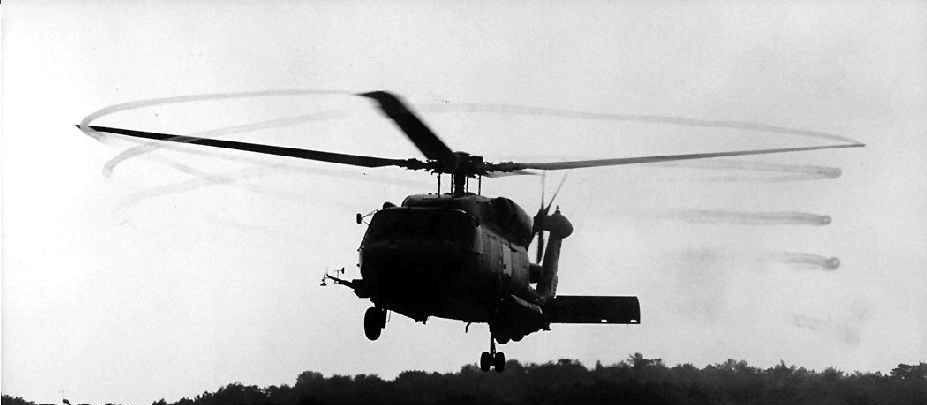
\includegraphics[width=0.9\textwidth]{figures/natural-condensation.png}\\
  \caption{通过自然凝结现象观察到的旋翼桨尖涡\upcite{Leishman1998}}
\end{figure}

为了在不具备自然凝结条件的时候也能对旋翼尾迹进行观察,喷烟法被引入旋翼空气动力学的研究中。
荷兰国家航空研究院\footnote{National Aeronautical Research Institute}的Drees等(1951)\upcite{Drees1951}
较早地利用该方法开展了旋翼流场的流动显示实验。
该实验通过在风洞引入喷烟装置,获得了直升机在悬停、前飞、下降等状态下旋翼附近的流动图像,并重点研究了旋翼处于涡环状态(Vortex Ring State, VRS)时的流动图像。
\begin{figure}[t!]
\begin{floatrow}
\ffigbox{\caption{利用喷烟法观察到的旋翼桨尖涡\upcite{Leishman1998}}}{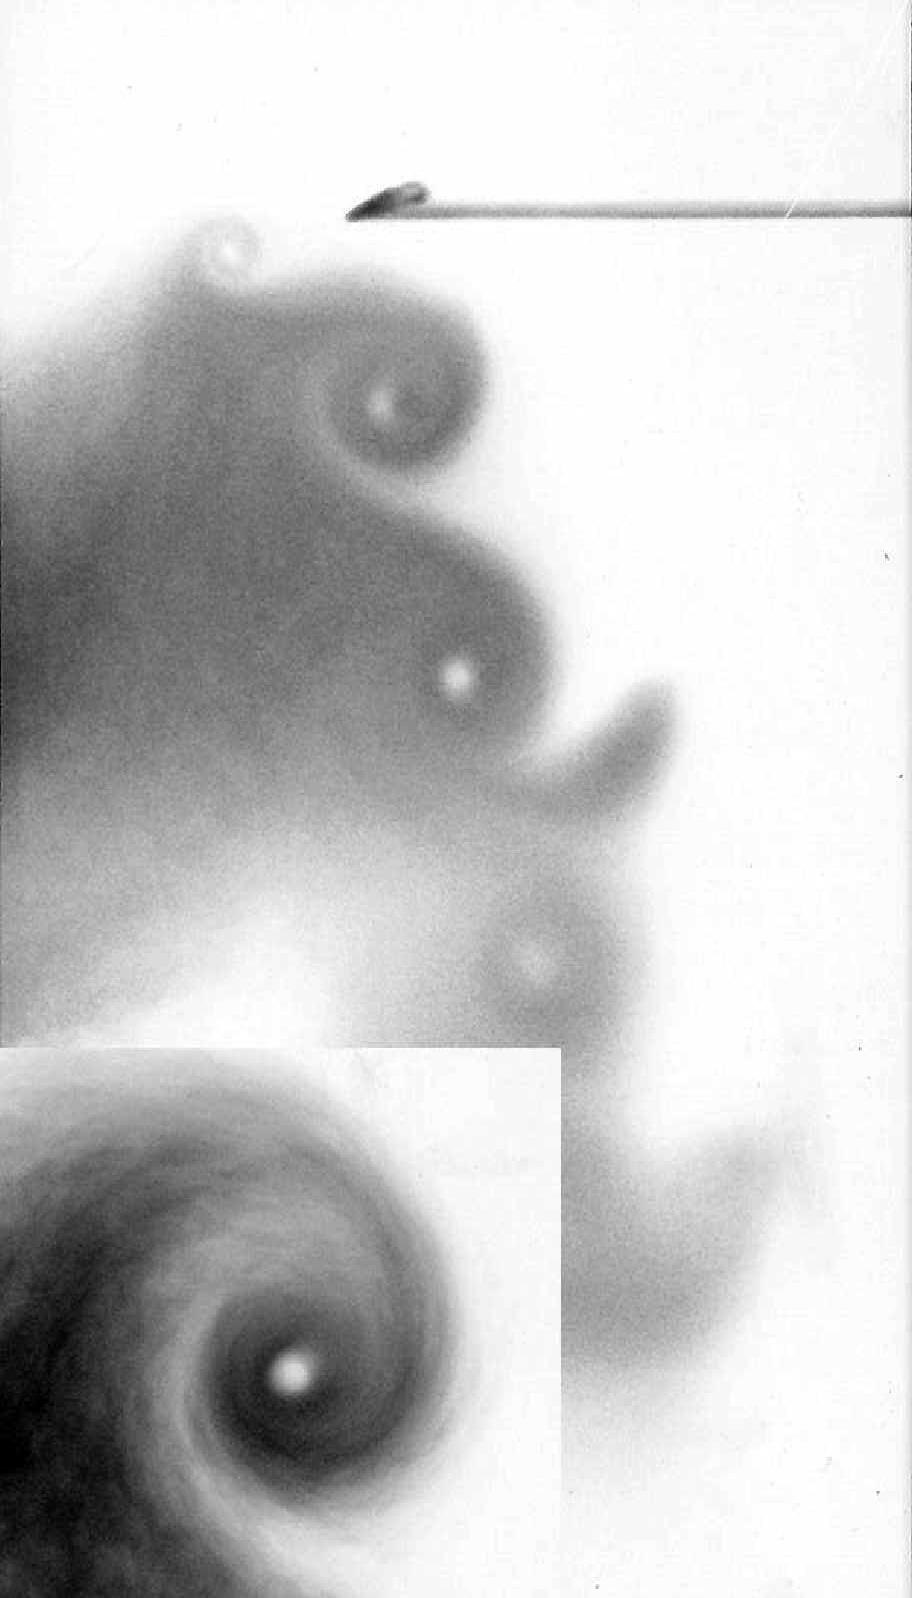
\includegraphics[width=0.45\textwidth]{figures/tip-vortex.jpg}}
\ffigbox{\caption{利用阴影法观察到的旋翼桨尖涡\upcite{Bagai1993}}}{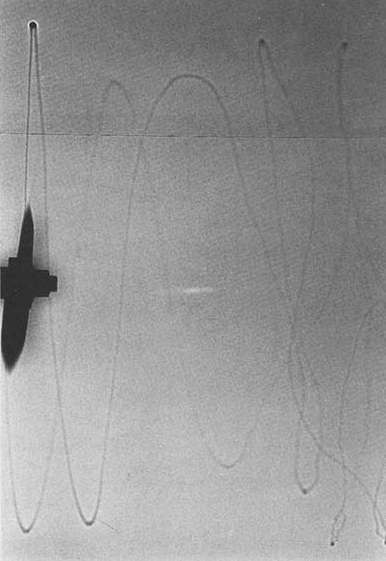
\includegraphics[width=0.45\textwidth]{figures/shadow.png}}
\end{floatrow}
\end{figure}

桨尖涡涡核区与背景流场的空气密度存在差别,对其光学特性(如折射率)有显著影响。
基于该原理和频闪摄影技术,人们发明了纹影法和阴影法,并将其引入旋翼空气动力学的研究中。
美国马里兰大学帕克分校\footnote{University of Maryland, College Park}的Bagai和Leishman(1993)\upcite{Bagai1993}
利用该方法研究了螺旋桨和旋翼桨尖涡的几何结构,观察到了旋翼尾迹的不稳定(非周期)现象。

定性实验虽然没有给出描述流场的各物理量的具体数值,但给出了各种飞行状态下的旋翼尾迹结构的物理图像,并初步验证了一些早期旋翼空气动力学理论(如滑流理论)的结论。
随着测量技术的进步,一些定性实验方法后来发展成为定量实验方法,或发展成为定量实验的一个前置环节。

\subsection{定量实验}
根据所测量的物理量以及对流场的刻画程度,可以将旋翼空气动力学定量实验大致分为两大类:
\begin{compactdesc}
  \item[测力实验]
  此类实验主要用于反映气流对旋翼影响的宏观效果。
  利用六分量天平、扭矩天平等仪器设备,可以对旋翼中心或全机参考点处的三个力分量和三个力矩分量进行测量。
  由于实验原理和实验设备都比较简单,所得的实验数据经过简单处理即可应用于结构动力学和飞行动力学分析,因此这类实验至今仍受到许多研究机构的重视。
  \item[测速实验]
  此类实验主要用于研究流场的流动细节。
  根据测量对象的范围,测速实验又可分为单点测量和多点测量两类。
  早期的单点测量实验主要采用热线测速仪(Hot Wire Anemometer)等介入式测量设备,测速探头本身对流场会造成一定干扰,因此测量结果不能完全反映真实流动情况。
  这一弊端后来被激光多普勒测速技术(Laser Doppler Velocimetry, LDV)所克服,但LDV仍属于单点测量技术。
  同属于非介入式测量技术的粒子成像测速技术(Particle Image Velocimetry, PIV),解决了多点同步测量的难题,能够实现对流场(流速)的高分辨率测量,
  目前已成为流体力学新发现的重要来源,也是验证数值计算方法的重要依据。
\end{compactdesc}

美国普林斯顿大学\footnote{Princeton University}的孙茂和Curtiss(1983)\upcite{Sun1983,Sun1989}
通过若干实验,研究了直升机低空低速飞行时地面效应对其气动性能的影响。
该组实验包括基于喷烟法的定性流动显示实验和基于热线测速仪的模型旋翼诱导速度分布定量测量试验。
结果显示,直升机低空低速飞行时,自由来流和地面将使旋翼尾迹向上卷起,从而显著影响旋翼气动载荷特性。
当卷起的尾迹接近桨盘平面并处于旋翼下方时,桨盘前侧诱导速度分布将发生较大幅度的不规则变化,从而引起旋翼气动力和气动力矩的不规则剧烈变化。

美国马里兰大学帕克分校的Leishman等(1996, 1998)\upcite{Leishman1996,Leishman1998a}
基于LDV,对桨尖涡切向和轴向速度、环量、黏性引起的涡核增大进行了测量,研究了旋翼尾迹的三维速度场;
对桨尖涡涡核位置进行了测量,研究了悬停状态桨尖涡的非周期现象。

%%%%%%%%%%%%%%%%%%%%%%%%%%%%%%%%
在国内,南航、北航等航空院校也开展了一些旋翼空气动力学方面的定量实验。

南京航空航天大学的唐正飞、高正等(1997, 1998)\upcite{Tang1997,Tang1998}
利用三维LDV,测量了共轴式双旋翼悬停状态的流场;为了对比,对单旋翼流场也进行了测量。
测量的物理量包括诱导速度沿三个方向(轴向、径向和周向)的分量,得到了两副旋翼尾迹相互交汇、干扰下的流动图像。

北京航空航天大学的邓彦敏等(2007, 2012)\upcite{Yu2007,Ma2012}
采用二维PIV,在水洞中对共轴式双旋翼悬停及不同前飞速度下的流场进行了测量,并对上下两副旋翼的气动干扰特性作了定量研究。
该实验测量了流场的瞬时涡量和速度分布、桨尖涡结构和脱落轨迹、尾迹边界等。
测量结果显示,共轴双旋翼悬停流场由上旋翼所主导;与单旋翼相比,双旋翼的尾迹结构更加不稳定。

以上定量实验结果,为旋翼气动设计提供了重要参考信息,也为验证分析模型和计算方法提供了参照对象。

\subsection{小结}
实验研究表明,旋翼流场具有以下关键特征\upcite{Leishman2006,Johnson2013}:
\begin{compactdesc}
  \item[桨尖涡主导]
  虽然流体力学界对于“涡”(vortex)的定义仍存在分歧\upcite{Tong2009},%p5
  但是无论根据何种定义,从实验事实中总能一致地识别出旋翼桨尖涡的存在。
  实验观测和数值计算都显示,旋翼高速旋转时,每片桨叶的桨尖和桨根处会各拖出一条集中涡。
  其中,桨根涡自生成后会迅速耗散并失去规则的涡结构,而桨尖涡自生成后则能在较长时间内保持强度和涡结构,因而主导着旋翼流场。
  定量研究进一步表明,桨尖涡的涡核半径很小,涡核内速度梯度较大,涡核外则接近无旋流动。
  这一流动特征对实验观测和数值计算在分辨率的空间配置上提出了不同的需求。
  \item[非定常]
  桨叶的固体表面对于空气流场而言,属于移动的壁面边界。
  通常,桨叶绕旋翼轴作周期运动时,描述其周围流场的各物理量的也随时间近似按周期变化。
  即使是悬停状态,虽然桨叶附近的空气流动接近定常状态,但是远离桨盘的桨尖涡也会因系统不稳定而表现出空间和时间的随机性。
  因此,非定常性是旋翼流场固有的特征,这决定了与旋翼相关的流动问题的研究难度往往要高于固定翼所对应的问题。
  \item[动态失速]
  通过简单的运动学分析可知,直升机处于前飞状态时,后行侧桨叶剖面的迎角大于前行侧,容易发生失速。
  另一方面,桨叶剖面的迎角随旋翼转动而周期变化,这种迎角的周期变化会导致翼型气动力出现时滞效应。
  这种动态失速现象,使得许多对固定翼行之有效的定常或准定常分析方法对旋翼不再适用。
  \item[局部可压缩]
  直升机旋翼桨尖速度的设计值通常为$0.7\sim0.9~M$,属于高亚音速范围,压缩性已较为明显。
  随着前飞速度增大,在前行侧桨叶桨尖处可能会出现局部跨音速区,甚至产生激波。
  桨叶的旋转又使得可压缩区域与低速不可压缩区域之间没有固定的、显著的界线。
  这一流动特征使得原本在固定翼空气动力学中已经形成的分别适用于不可压缩和可压缩流动的分析方法,需经过特殊处理才能应用于旋翼空气动力学的研究。
\end{compactdesc}

上述旋翼流场所固有的流动特征,使得旋翼空气动力学的研究难度明显大于固定翼空气动力学。
除此之外,以下在直升机各种常见工作状态中普遍存在的气动干扰现象也增加了问题的复杂程度:
\begin{compactdesc}
  \item[桨-涡干扰]
  在下降、俯冲、大机动等飞行条件下,或对于桨盘面积有重叠的双旋翼构型,桨尖涡与桨叶之间不可避免地会发生碰撞。
  桨尖涡经过桨叶时,桨叶表面的压力分布受到强烈扰动,从而成为旋翼振动和噪声的重要来源。
\begin{figure}[t!]
    \centering
    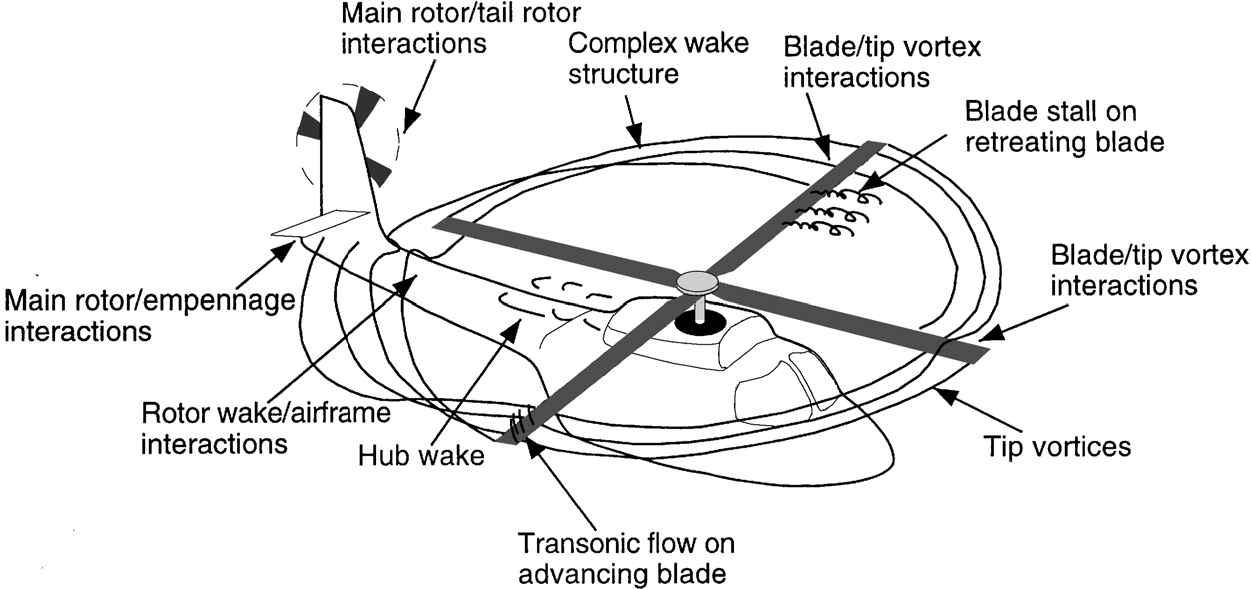
\includegraphics[width=\textwidth]{figures/aero-interaction.jpg}
    \caption{直升机气动干扰示意图\upcite{Leishman1998}}
\end{figure}
  \item[旋翼-机身干扰]
  通常,直升机机身处于旋翼的下游区域,对旋翼尾迹起阻挡作用。
  旋翼拉力、悬停气动效率这些重要的总体性能指标将受到影响。
  另一方面,桨尖涡以一定频率与机身发生碰撞,使得机身表明的压力分布受到扰动,从而成为机体振动的重要来源。
  \item[旋翼-固定翼干扰]
  直升机上除了旋翼以外,一般还有水平尾翼、垂直尾翼等固定翼面,用于增加飞行稳定性,或提供额外的操纵面。
  当这些固定翼面受到旋翼尾迹扰动时,其上感知的气动力有别于相应孤立部件在相同自由来流条件下所感知的气动力,从而会影响全机的配平和稳定性。
  \item[旋翼-地面干扰]
  当直升机从地面起飞或贴地低空飞行时,地面的阻挡将改变旋翼尾迹的流向。
一般而言,地面效应会使旋翼拉力、悬停气动效率等总体性能指标有所提升;
  但在地面存在大量砂石等颗粒物的条件下,地面效应会进一步引发沙盲现象(图\ref{brownout}),导致飞行员视线受到遮挡,从而影响飞行安全。
\begin{figure}[t!]
    \centering
    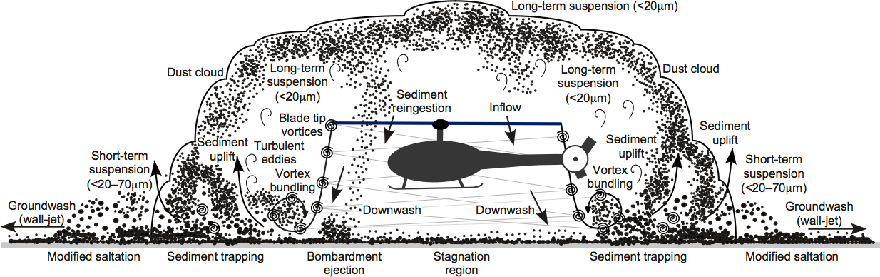
\includegraphics[width=\textwidth]{figures/brownout.png}
    \caption{沙盲现象示意图\upcite{Syal2012}}\label{brownout}
\end{figure}
  \item[旋翼-舰面干扰]
  对于舰载直升机,旋翼与舰面和水面之间也存在类似于地面效应的气动干扰现象。
  舰面与水面的高度差造成二者对旋翼干扰程度的不同,会使得旋翼经过甲板边缘时,桨盘上升力分布发生突变,从而改变直升机的姿态。  
  此外,当海面风速较大或舰艇高速航行时,舰桥等结构对自由来流的扰动,会在直升机起降平台上产生紊乱的空气尾流,从而增加直升机起降的难度。
  由于直升机在舰面起降时相对速度较低,旋翼尾迹与船体空气尾流相互影响,舰面气流对其飞行的影响较之固定翼飞机显得更加突出。
\end{compactdesc}

以上旋翼流场特有的关键特征和直升机特有的气动干扰现象,始终是旋翼空气动力学研究的关键问题。
许多在固定翼空气动力学中得到成功应用的方法,在应用到旋翼空气动力学研究之前,必须经过适当的改造;
旋翼空气动力学本身也产生了一些特有的分析模型和数值计算方法,并且还在不断发展和改进。

\section{旋翼空气动力学(数值计算)}

\subsection{入流模型}
入流(Inflow)模型描述的是旋翼尾迹在桨盘平面处的诱导速度(入流)与旋翼气动力之间的数量关系。

滑流理论,又称动量理论,是最早的也是最简单的入流模型。
该理论基于作用盘(Actuator Disk)模型和动量定理,给出的悬停状态下桨盘平面的诱导速度为\upcite{Johnson1994}:
\begin{equation}
  v_{ \mathrm{0} }  = \sqrt{\frac{C_\mathrm{T}}{2}}
\end{equation}
其中,$C_\mathrm{T}$是旋翼拉力系数,$v_{ \mathrm{0} }$是无量纲诱导速度。
该模型只给出了沿桨盘平面均匀分布的诱导速度场,并且属于静态(准定常)入流模型,所以通常只在初步设计阶段用来进行旋翼性能估算。

此后,各种改进的静态入流模型不断被提出,桨盘平面诱导速度分布的非均匀性得以体现。
在此基础上,出现了一阶状态空间方程形式的动态入流模型,以考虑旋翼气动力与入流关系的非定常性,其中最具代表性的是Pitt-Peters动态入流模型。
该模型包含三个无量纲诱导入流分量:均匀入流分量$v_{\mathrm{0}}$,横向入流分量$v_{\mathrm{s}}$和纵向入流分量$v_{\mathrm{c}}$。
桨盘上任意一点的无量纲诱导速度可以写为无量纲展向位置$r$ 和气流方位角$\psi$ 的函数:
\begin{equation}
v = v_0 + v_{\mathrm{c}} r \cos \psi + v_{\mathrm{s}} r \sin \psi
\end{equation}
这三个无量纲诱导速度分量和它们的无量纲时间导数,与桨盘的三个无量纲气动力$C_{ \mathrm{T} },C_{ \mathrm{L} },C_{ \mathrm{M} }$之间的关系,可以写成状态空间形式:
\begin{equation}
\begin{bmatrix} M \end{bmatrix}
\overset { * }{ \begin{pmatrix} v_{ \mathrm{0} } \\ v_{ \mathrm{s} } \\ v_{ \mathrm{c} } \end{pmatrix} }
+
\begin{bmatrix} L  \end{bmatrix}^ { -1}
\begin{pmatrix} v_{ \mathrm{0} } \\ v_{ \mathrm{s} } \\ v_{ \mathrm{c} } \end{pmatrix}
=
\begin{pmatrix} C_{ \mathrm{T} } \\ C_{ \mathrm{L} } \\ C_{ \mathrm{M} } \end{pmatrix}
\end{equation}
文献\cite{Chen1989}对截至到上世纪80年代末的各种静态和动态入流模型作了详细的综述。

1989年,美国佐治亚理工学院\footnote{Georgia Institute of Technology}的He(1989)\upcite{He1989,Peters1995}
基于势流理论,又提出了广义动态尾迹模型(Peters-He有限状态入流模型),将状态变量个数推广到任意多,进一步体现了高阶谐波的影响。

值得注意的是,经典的动量理论模型被作为准静态情况的特例包含在Pitt-Peters动态入流模型之中,
Pitt-Peters动态入流模型又是Peters-He有限状态入流模型在状态变量取到一阶时的特例。

动态入流模型具有形式紧凑、计算效率高的优点,在直升机飞行动力学建模\upcite{Yang1996,Sun2001}和旋翼气动弹性问题\upcite{Panda1985,Jang1988}的研究中得到了广泛的应用。

但是,所有的入流模型都是从作用盘模型出发,引入尾迹形状规则且无限延伸等理想化假设,最后得到气动力与入流系数的关系。
显然,这种简单的物理模型无法真实反映旋翼流场由桨尖涡主导、局部可压缩等特性,也无法处理存在复杂气动干扰的问题,目前正逐步被更接近物理真实的自由尾迹模型取代。

\subsection{涡线尾迹模型}
涡线尾迹模型是用于描述旋翼尾迹中涡量空间分布情况的物理模型,在一些文献中也用来指代该物理模型所对应的数值计算方法。
该模型的基本思想是用直线或曲线涡元(涡线单元)对涡量场进行离散,通过研究涡线单元的运动和演化来描述涡量场,属于连续介质力学中的拉格朗日观点(质点系观点)\upcite{Fung1994}。
得到涡量场后,再利用Biot-Savart定律对涡量场进行积分,从而得到诱导速度场。

从发展历程来看,涡线尾迹模型经历了刚性尾迹,预定尾迹和自由尾迹三个阶段。

\subsubsection{刚性尾迹模型}
刚性尾迹(Rigid Wake,又译“固定尾迹”)模型假设旋翼尾迹中的涡量集中分布在以桨盘为底面的直圆柱面或斜圆柱面上,或集中分布在从桨尖拖出的螺旋线上。
此模型中,涡系的几何形状只受自由来流和平均入流的驱动,不因涡系自诱导和互诱导而发生变形,因而被称为“刚性(Rigid)”尾迹。
由于刚性尾迹的几何形状简单,经过一些数学推导,有时可以得出初等函数、特殊函数或级数形式的解。

北京航空航天大学的陈铭(2004)\upcite{Chen2003,Chen2004,Chen2005}
利用刚性尾迹模型,将旋翼用与无限片桨叶等效的作用盘代替,对共轴双旋翼前飞气动特性进行了研究,得到了解析形式的诱导速度解。

虽然根据刚性尾迹模型得出的解析形式的解在计算机上能够快速得出数值结果,但其所假设的尾迹几何结构与实际情况相差较大。
尤其是在大机动、贴地飞行等条件下,尾迹畸变严重,刚性尾迹模型不再适用。
目前,刚性尾迹模型只被用于对计算机时要求极高的实时仿真程序,或用于为自由尾迹模型、CFD计算程序提供迭代初值。

\subsubsection{预定尾迹模型}
预定尾迹(Prescribed Wake)模型在刚性尾迹模型的基础上,根据一些特殊旋翼在特殊状态下的实验结果,引入一些参数对刚性尾迹的几何形状进行修正。
美国陆军航空机动研究与发展实验室\footnote{U.S. Army Air Mobility Research and Development Laboratory}
的Landgrebe(1971)\upcite{Landgrebe1971}通过水洞试验,提出了一种半经验的旋翼尾迹模型。
但该模型的适用性严重依赖于根据个别实验确定的经验参数,普适性较差,并没有从根本上解决刚性尾迹模型无法准确描述尾迹几何结构的问题。

\subsubsection{自由尾迹模型}
自由尾迹(Free Wake)模型允许涡元像流体微团一样在流场中自由运动。
这里的“自由”是指相对于刚性尾迹和预定尾迹,自由尾迹不再对尾迹几何结构进行限制,涡元(流体微团)的运动仍然受流体力学基本原理支配。
“涡元像流体微团一样在流场中自由运动”即是指涡元运动满足如下关系:
\begin{equation}\label{ODE}
\frac{\mathrm{d}\symbfit{r}}{\mathrm{d} t} = \symbfit{u} = \symbfit{u}_{\mathrm{\infty}}+\symbfit{u}_{\mathrm{ind}}
\end{equation}
其中,$\symbfit{r}$是涡元位置,$\symbfit{u}_{\mathrm{\infty}}$是自由来流速度,$\symbfit{u}_{\mathrm{ind}}$是旋翼涡系对该点的诱导速度。
该诱导速度需根据Biot-Savart定律\upcite{Anderson2001}计算得到。
考虑$A$、$B$两点之间一段强度为$\Gamma$的涡线,它对空间任意一点$C$的诱导速度由以下积分给出:
\begin{equation}
\symbfit{u}_{\mathrm{ind}}^{C}
=
\int_{A}^{B}
\frac{\Gamma}{4\pi}
\frac{\mathrm{d} \symbfit{l}\times\symbfit{r}}{r^3}
\end{equation}
引入涡线模型离散后,\ref{ODE}式变为一个高度非线性的常微分方程系统,求解的难度来源于非线性的诱导速度项$\symbfit{u}_{\mathrm{ind}}$。

自由尾迹模型所依据的“涡元像流体微团一样在流场中自由运动”,
实际上是Kelvin定理\footnote{在理想流体中,沿一条封闭物质线的速度环量不随时间变化\upcite{Cottet2000}。}应用到理想流体时的一个推论,
因而自由尾迹模型的成立条件是流体无黏、正压且外力有势。
在旋翼尾迹问题中,外力(重力)可以忽略,流体(空气)满足正压条件,但黏性通常不可忽略,为此需引入黏性涡核模型\upcite{Leishman2006}进行修正。
该模型可进一步分有限涡核模型和涡核演化模型两部分。
简单的集中涡线模型存在奇异性,为消除这种奇异性,通常以一个截面半径为有限值的涡管代替截面半径为零的集中涡线。
在有限涡核模型的基础上,令涡核半径随涡龄的增长而变大,以此来体现空气粘性引起的涡量耗散效应,涡核以外的流体则认为是无粘的。

最早尝试利用自由尾迹模型对旋翼流场进行建模的有
美国麻省理工学院\footnote{Massachusetts Institute of Technology}的Scully(1967, 1975)\upcite{Scully1967,Scully1975},
美国陆军的Landgrebe(1969)\upcite{Landgrebe1969}等。
早期的自由尾迹算法普遍存在收敛性差的问题,此后一段时间,许多学者在改善该模型的收敛性方面做了大量工作。

美国普林斯顿大学的孙茂和Curtiss(1983)\upcite{Sun1983,Sun1989a}
建立了一种简化的自由尾迹卷起模型,用以研究旋翼尾迹与地面的相互影响,并在此基础上计算了桨盘平面的诱导速度分布。
结果显示,地面和卷起涡显著地改变了旋翼近尾迹的几何形态,从而造成了桨盘平面诱导速度分布的剧烈变化。

美国马里兰大学帕克分校的Leishman教授及其研究团队,于上世纪90年代提出和改进了多种自由尾迹算法。

Crouse Jr.和Leishman(1993)\upcite{Crouse1993}
提出了一种预估校正格式(Predictor-Corrector scheme, PC),用于提高的收敛性,控制计算量。
该算法采用两点中心差分格式对涡量场进行时间和空间离散,通过引入周期条件确保稳态解收敛。
但对悬停状态客观存在的非周期解,无法给出正确的计算结果。

Bagai和Leishman(1995)\upcite{Bagai1995,Bagai1995a,Bagai1996}
提出了一种伪隐式预估校正积分格式(Pseudo-Implicit Predictor-Corrector Integration scheme, PIPC),用于求解存在稳态周期解的旋翼尾迹问题。
该算法采用五点中心差分格式对涡量场进行时间和空间离散,利用松弛迭代法和周期条件改善解的收敛性。
基于该算法,作者计算了单旋翼、双旋翼构型的直升机在悬停、低速前飞、高速前飞等各种飞行状态中的旋翼尾迹,结果很好地反映了旋翼尾迹的畸变。
但该方法用到了周期条件,因而只适用于存在稳态周期解的问题;但也有学者质疑稳态周期解的存在\upcite{Kini2002}。
另外,参数分析表明,解的收敛性和尾迹几何结构与部分经验参数的选取有关,使该方法的通用性受到质疑。

Bhagwat和Leishman(2000, 2002, 2004)\upcite{Bhagwat2000,Bhagwat2000a,Leishman2002,Leishman2004}
提出了一种时间精确(Time Accurate)自由尾迹模型,用于分析旋翼尾迹的动态响应过程。
该算法采用二阶后向差分预估校正格式(Predictor-Corrector 2nd-Backward, PC2B),提高了算法的数值稳定性。
由松弛迭代法(如Bagai的PIPC格式)给出初始条件后,可以沿时间积分尾迹方程和桨叶动力学方程,得到旋翼尾迹和桨叶运动的动态响应值。
基于该算法,作者计算了多种旋翼构型在不同飞行条件下的尾迹几何形态,研究了旋翼作机动时的尾迹瞬态变化过程,并对涡环状态这一典型的不稳定状态进行了模拟。
该模型在以上算例中均给出了很好的结果。
\begin{figure}[t!]
    \centering
    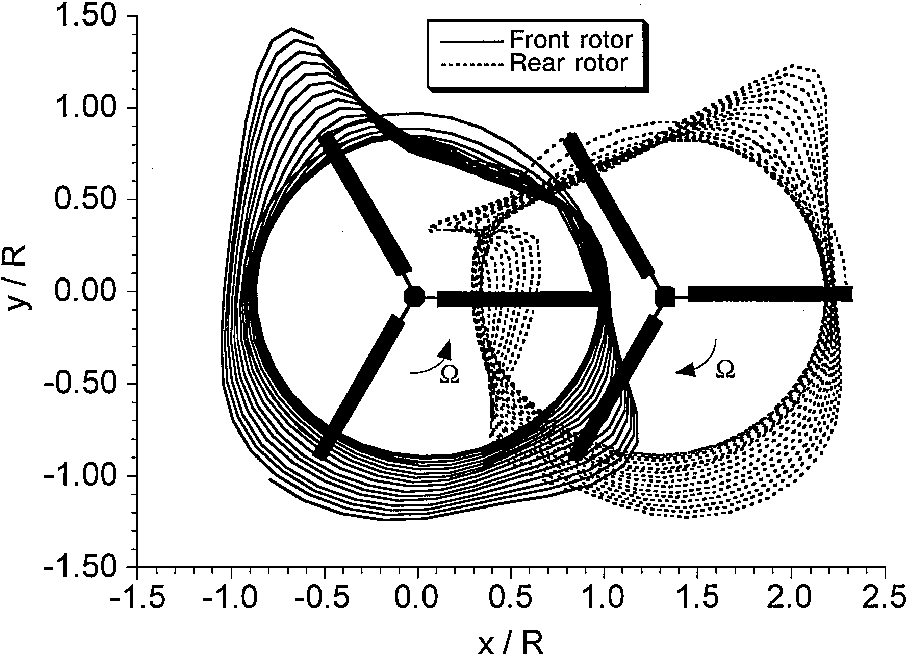
\includegraphics[height=0.3\textheight]{figures/free-wake.png}
    \caption{利用自由尾迹模型计算得到的纵列式双旋翼尾迹\upcite{Leishman2002}}\label{free-wake}
\end{figure}

Gupta和Leishman(2006)\upcite{Gupta2006}
将上述时间精确自由尾迹模型应用到风力机械的气动性能研究中。
%
Ananthan和Leishman(2006)\upcite{Ananthan2006}
基于时间精确自由尾迹模型,研究了机动飞行状态下的旋翼尾迹几何形态和涡量分布,初步研究了桨涡干扰引起的旋翼噪声。
Ribera和Celi(2007)\upcite{Ribera2007}
也利用该模型开展了直升机飞行动力学方面的研究。

美国俄亥俄州立大学\footnote{Ohio State University}的Conlisk教授也开展了一些自由尾迹模型算法方面的研究\upcite{Conlisk2001}。

Jain和Conlisk(2000)\upcite{Jain2000}
采用升力线理论对桨叶进行建模,采用时间步进(Time-Stepping)自由涡方法对桨尖涡运动进行计算。
在做时间步进积分时,此文采用了数值稳定的四阶隐式Adams–Moulton格式。
基于上述方法,作者通过数值计算研究了在实验中观察到的两条桨尖涡之间相互缠绕的现象。

Kini和Conlisk(2002)\upcite{Kini2002}
采用与\cite{Jain2000}中类似方法研究了悬停状态桨尖涡几何结构的稳定性。
计算结果显示,悬停状态时,桨尖涡几何结构的周期性条件只对前几圈桨叶适用,后几圈的桨尖涡几何结构表现出明细的时间非周期性。
由于采用了数值稳定的隐式Adams–Moulton格式,并且在步长小于$4~\deg$时可以给出足够精确的结果,
作者认为,物理不稳定是导致悬停状态桨尖涡远场尾迹非周期结构的主要原因,而非算法的数值稳定性问题。
这与Bagai和Leishman(1995)\upcite{Bagai1995,Bagai1995a,Bagai1996}之前所提出的观点相反。

Pulla和Conlisk(2006)\upcite{Pulla2006}
基于时间步进自由尾迹方法研究了地面效应影响下的直升机气动特性。
其中,旋翼尾迹通过自由涡方法进行建模,桨叶气动力由升力面理论给出,地面则采用镜像法进行处理。
时间步进算法采用与\cite{Jain2000,Kini2002}中类似的Adams-Moulton格式。
计算结果与佐治亚理工的实验数据进行了对比,验证了算法的可行性。

%%%%%%%%%%%%%%%%%%%%%%%%%%%
在国内,自由尾迹模型也有相应的发展和应用。

南京航空航天大学的李春华和徐国华(2007)\upcite{Li2007}
基于时间精确自由尾迹模型,研究了倾转旋翼的气动特性。
%
李攀和陈仁良(2010)\upcite{Li2010}
基于时间精确自由尾迹模型,提出了一种新的差分格式,建立了一种高置信度的直升机飞行动力学模型。

北京航空航天大学的陈铭等(2014)\upcite{Wang2014}
基于稳态自由尾迹模型,研究了旋翼几何参数对共轴双旋翼悬停性能的影响。
%
曹义华等(2015)\upcite{Lv2015}
采用自由尾迹模型和面元法,分别对旋翼和机身进行建模,建立了一种旋翼-机身气动干扰模型,并进行了配平计算。

尽管自由尾迹模型仍然是目前直升机工程界普遍认可的旋翼空气动力学分析手段,但该模型本身也存在一定的局限性。
首先,自由尾迹模型必须与其他模型(如升力面模型)配合,才能获得桨尖涡环量的初始值。
其次,目前常用的涡核模型都存在若干经验参数,并且桨尖涡的截断位置也需要人工设置。
另外,这种物理模型虽然能够大体上还原桨尖涡的几何结构,但在处理桨尖涡与固体壁面碰撞等问题时,只能采取回避或作镜像处理的方法,无法描述涡结构破碎等现象。
因此,自由尾迹模型还不是一种十分完备的物理模型。

\subsection{黏性涡粒子模型}\label{Viscous-Vortex-Particle-Method}
黏性涡粒子模型(Vortex Particle Model, VPM)与自由尾迹模型类似,也属于基于拉格朗日观点的分析模型。
所不同的是该模型用涡粒子代替了涡线,每个涡粒子由位置$\symbfit{x}$和涡量$\symbfit{\omega}$两个矢量来描述。
其中,涡元位置$\symbfit{x}$的变化规律与自由尾迹模型一样,由如下简单的运动学关系描述:
\begin{equation}\label{}
\frac{\mathrm{d} \symbfit{x}}{\mathrm{d} t}
=
\symbfit{u}
\end{equation}
而涡量$\symbfit{\omega}$的变化规律则由涡量输运方程给出。

旋翼尾迹流场属于低亚音速流动,通常可以对空气采用各项同性、不可压缩、正压等理想化假设。
基于这些假设,可以将Navier-Stokes方程(详见\ref{Navier-Stokes-Equation})简化为:
\begin{equation}\label{}
%\frac{\mathrm{D} \symbfit{u}}{\mathrm{D} t}
%=
\frac{\partial \symbfit{u}}{\partial t}
+
\left( \symbfit{u}\cdot\nabla \right) \symbfit{u}
=
-\frac{1}{\rho} \nabla p
+
\nu \nabla^2 \symbfit{u}
+
\symbfit{f}
\end{equation}
利用矢量分析公式\upcite{Zorich2004}、%\footnote{参见附录\ref{vector}}、
涡量定义\footnote{$\symbfit{\omega}=\nabla\times  \symbfit{u}$}、
不可压\footnote{$\nabla\cdot  \symbfit{u} = 0$}、
正压\footnote{$\nabla \rho \times \nabla p = \symbfit{0}$}、
体积力有势\footnote{$ \symbfit{f} = -\nabla V  $}等条件,
可将上式改写成涡量形式:
\begin{equation}\label{Vorticity-Transport-Equation}
%\frac{\mathrm{D} \symbfit{\omega}}{\mathrm{D} t}
%=
\frac{\partial \symbfit{\omega}}{\partial t}
+
\left( \symbfit{u}\cdot\nabla \right) \symbfit{\omega}
=
\symbfit{\omega} \cdot \nabla\symbfit{u}
+
\nu \nabla^2 \symbfit{\omega}
\end{equation}
该式左端为涡元涡量的物质导数,右端第一项表示涡元变形(拉伸、弯曲)的影响,右端第二项表示黏性引起的涡量扩散。
此即不可压缩、正压流体的涡量输运方程。

美国先进旋翼飞行器技术公司\footnote{Advanced Rotorcraft Technology, Inc.}的He等(2009)\upcite{He2009}
利用黏性涡粒子方法研究了旋翼尾迹中涡量的输运和扩散现象。
该方法避免了基于欧拉观点的数值离散方法所引入的数值耗散。
为提高计算效率,采用了TreeCode加速算法和快速多级子方法推高计算效率。
计算结果显示:
黏性涡粒子模型可以精确模拟旋翼尾迹在悬停、前飞等状态下的动态变化;
不借助经验参数,很好地捕捉到了尾迹收缩、桨尖涡卷起、涡量扩散等物理现象;
尾迹对总距突增操纵的动态响应计算结果与实验吻合很好。
此文中的旋翼尾迹初始涡量由升力线模型获得。
作者指出了用CFD方法替代该模型的可能性,但没有进一步给出具体实施方法和计算结果。

南京航空航天大学的魏鹏、徐国华等(2012)\upcite{Wei2012,Wei2012a}
基于黏性涡粒子模型,建立了一种适用于旋翼非定常流场特性分析的数值方法。
桨叶附着涡以及新生涡环量由Weissinger-L升力面模型\upcite{Weissinger1947}给出。
计算结果显示,该方法与自由尾迹方法和CFD方法相比,能够在兼顾效率的同时,更好地捕捉旋翼尾迹运动。
但升力面模型只适用于势流,并不能很好反映动态失速、桨尖激波等现象。
\begin{figure}[t!]
    \centering
    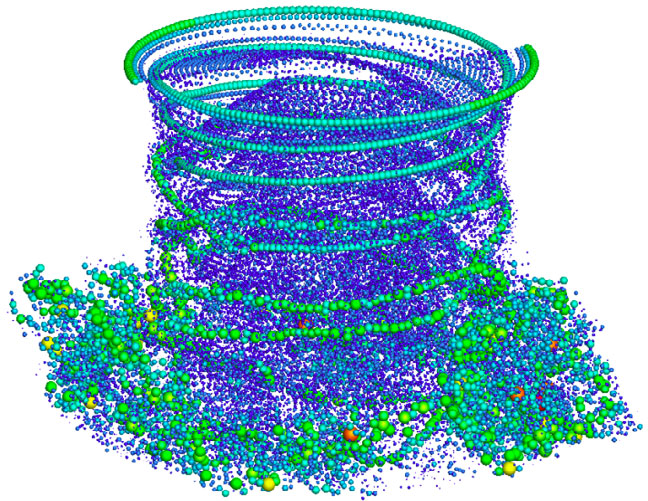
\includegraphics[height=0.3\textheight]{figures/vortex-particle.png}
    \caption{利用黏性涡方法计算得到的涡元分布\upcite{Wei2012}}\label{vortex-particle}
\end{figure}

清华大学的王浩文等(2014)\upcite{Tan2014}
采用非定常面元法、黏性涡粒子法及涡量镜面法,建立了旋翼-平尾非定常气动干扰分析模型。
计算结果显示,此方法计算精度高于时间精确自由尾迹,计算效率高于CFD。
但面元法只适用于势流,并不能真实反映桨叶表面的分离、压缩性等流动现象。

从上述研究内容来看,黏性涡粒子模型本身可以比较高效(与CFD相比)且精确(与自由尾迹相比)地捕捉旋翼尾迹中的典型流动现象;
但在处理桨叶、机身、固定翼面等壁面时,需引入其他模型作为补充。
除上面提到的只适用于势流的升力线模型、升力面模型、面元法外,也有研究人员尝试采用CFD方法对近壁面进行处理。

美国国家航空航天研究所\footnote{National Institute of Aerospace}的Anusonti-Inthra等(2008)\upcite{Anusonti-Inthra2008}
将雷诺平均Navier-Stokes方程方法(Reynolds-Averaged Navier-Stokes, RANS)与基于粒子的涡量输运方法(Particle-based Vorticity Transport Method, PVTM)进行耦合,
用于分析固定孤立机翼低速飞行时的气动性能和尾迹特性,并通过与风动实验数据进行对比,对该计算模型进行了验证。
该耦合方法将流场按主要流动特性,分为近壁面和远场区域,分别用三维可压缩RANS方法和PVTM方法进行求解。
计算结果显示,该耦合方法可以对机翼翼梢的三维流动效应进行合理的模拟,并且有效解决了常规RANS方法存在的数值耗散问题。
但也有研究人员认为,耦合方法本身及不同计算区域数据交换带来的复杂性,可能会抵消一部分涡粒子模型对计算效率的提升\upcite{Kamkar2011}。

\subsection{基于欧拉观点的涡量输运模型}\label{Vorticity-Transport-Model}
该方法基于欧拉观点(场观点),直接对涡量输运方程(\ref{Vorticity-Transport-Equation}式)进行数值求解。
从离散方法的角度看,该方法属于有限体积法,但描述流场的变量为涡量。
由于采用了涡量形式的问题表述形式,该方法能够有效地减小数值耗散引起的涡量非物理扩散。
涡量输运方法的主要弊端是难以处理壁面边界条件,无法考虑空气压缩性,因而必须引入其他方法(升力线、升力面、CFD等)作为补充。

英国的Brown,先后在格拉斯哥大学\footnote{University of Glasgow}和帝国理工学院\footnote{Imperial College, London}开展了一系列基于涡量输运方程的旋翼空气动力学数值计算研究。
在格拉斯哥大学期间,Brown(2000)\upcite{Brown2000}
采用基于欧拉网格的涡量守恒形式的Navier–Stokes方程(即涡量输运方程),计算了孤立旋翼和共轴双旋翼周围的非定常气动环境,并与实验数据进行了验证。
由于涡量输运方程不能直接处理壁面边界条件,此文通过升力线方法给出尾迹初始涡量。

格拉斯哥大学的Houston和Brown(2000, 2003)\upcite{Brown2000a,Houston2003}
采用有限状态入流模型与涡量输运模型两种方法,研究了直升机配平、自转下滑状等飞行力学问题。
计算结果表明,当自转下滑率较小时,两种模型给出的计算结果差别不大;随着下滑角增大,两者的差别逐渐变得明显。

帝国理工学院的Whitehouse与Brown(2003)\upcite{Whitehouse2003}
将涡量输运方法应用到大型固定翼飞机尾涡与直升机尾迹气动干扰问题的研究中。
计算结果显示,直升机高速飞行时,飞机尾涡不会对其造成严重影响;
但在低速飞行时,飞机尾涡会引起旋翼气动载荷和气弹响应的震荡,从而增加飞行员操纵的难度。

在帝国理工学院期间,Brown与Line(2005)\upcite{Brown2005}
对涡量输运方法进行了改进,使其计算效率得到提高。
新算法引入了一种半拉格朗日型(Semi-Lagrangian)自适应网格系统,在尽可能避免产生额外计算量的前提下,显著提高了计算结果的空间分辨率。
同时,该网格系统避免了在处理计算区域边界附近尾迹截断时需借助数值边界条件的问题。
另外,在应用Biot-Savart定律计算速度场时,采用快速多极子方法显著提高了计算效率。
对于壁面边界条件,此文仍借助升力线模型进行处理。
\begin{figure}[t!]
    \centering
    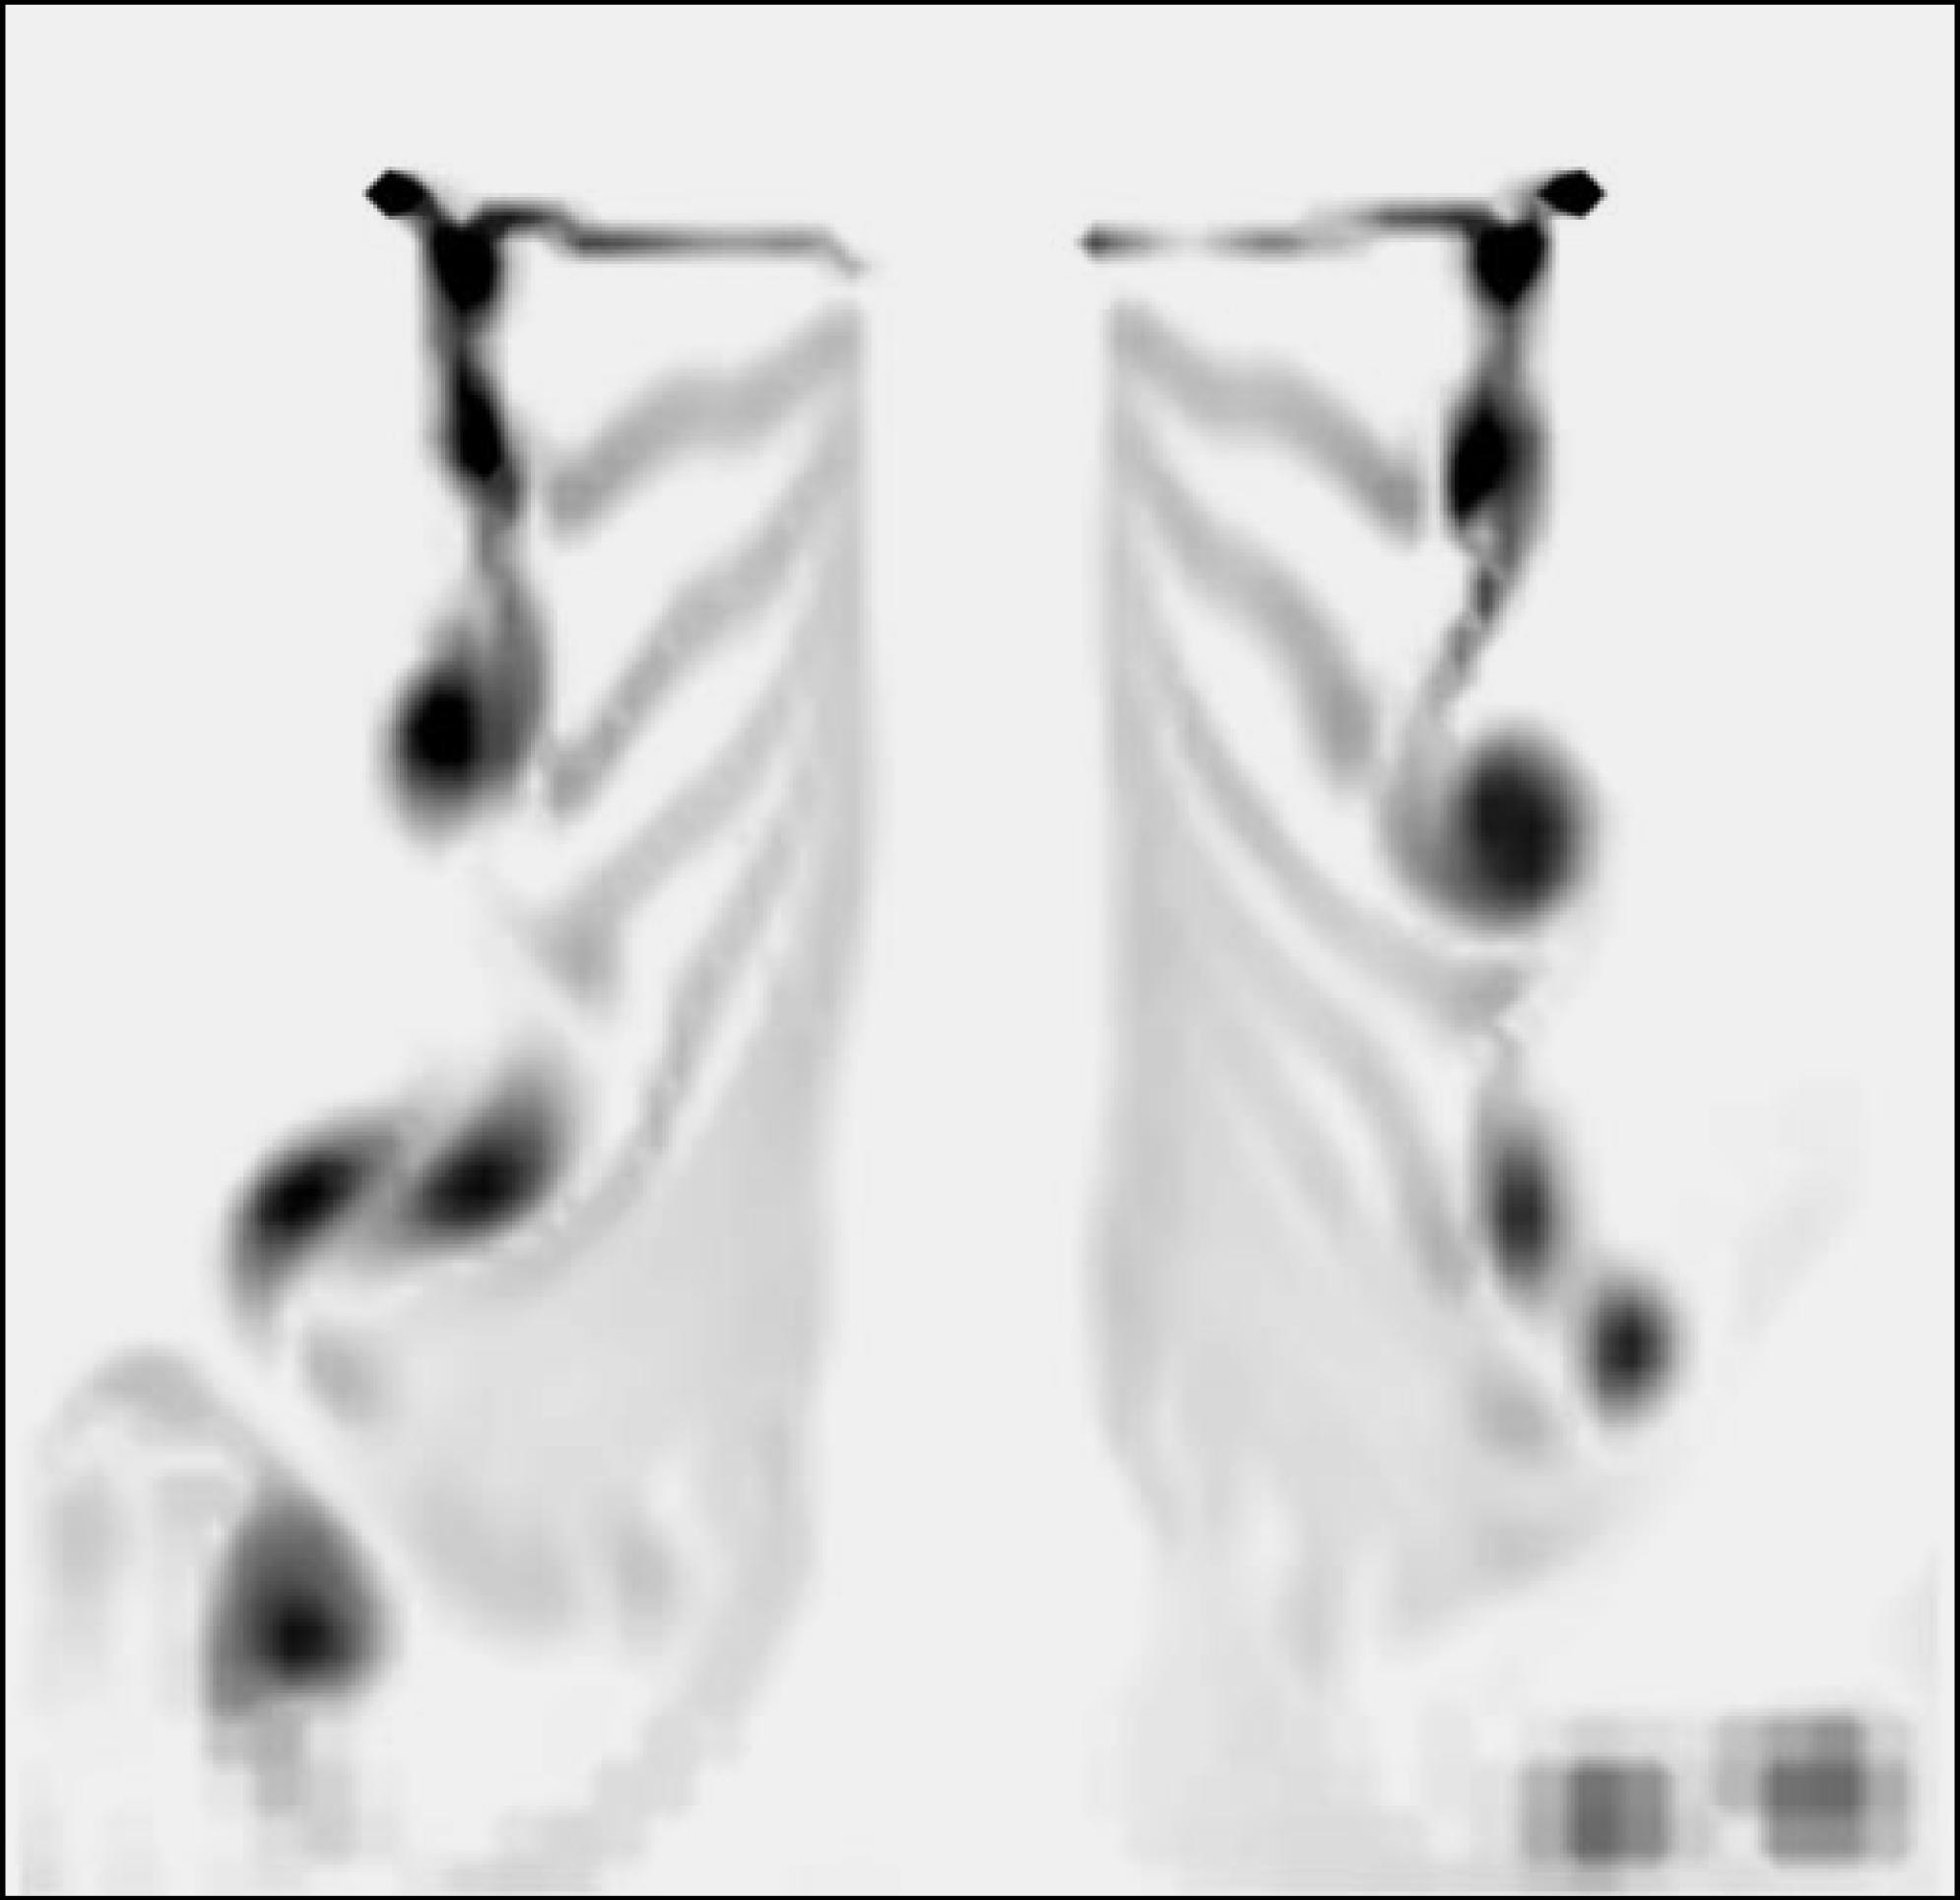
\includegraphics[height=0.3\textheight]{figures/vtm.jpg}
    \caption{由涡量输运方法计算得到的涡量分布\upcite{Brown2005}}\label{vtm}
\end{figure}

美国连续介质动力学公司\footnote{Continuum Dynamics, Inc.}的Whitehouse等(2007)\upcite{Whitehouse2007}
将涡量输运方程与Navier-Stokes方程相结合,建立了一种更加接近物理真实的旋翼空气动力学分析模型。
该模型采用基于原始变量(速度、压力)的Navier-Stokes方程对桨叶附近的流动情况进行描述,可以体现这一区域存在的空气黏性、压缩性等势流模型无法很好处理的流动特性;
对涡流主导的尾迹部分则采用基于欧拉观点的涡量输运方程进行描述,可以有效降低常规CFD方法造成的涡量非物理扩散。
利用该耦合模型,此文给出了一些固定翼、钝体、直升机上的算例,在流动特性捕捉和非定常载荷计算方面都给出了较好的结果。
\begin{figure}[t!]
    \centering
    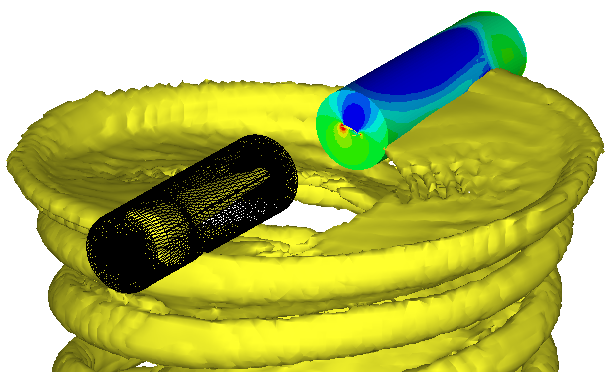
\includegraphics[height=0.25\textheight]{figures/whitehouse.png}
    \caption{涡量输运方程和Navier-Stokes方程耦合模型\upcite{Whitehouse2007}}
\end{figure}
\begin{figure}[t!]
    \centering
    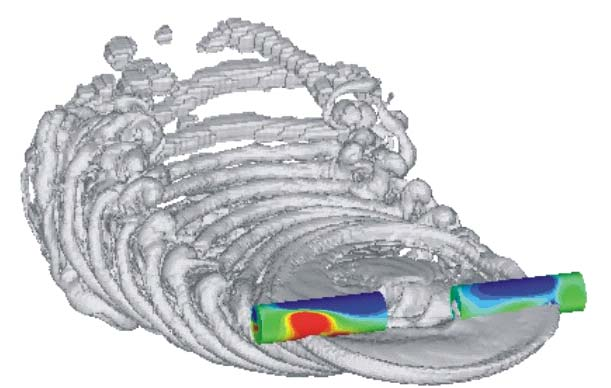
\includegraphics[height=0.25\textheight]{figures/whitehouse1.png}
    \caption{由涡量输运方程和Navier-Stokes方程耦合模型计算得到的前飞状态涡量分布\upcite{Whitehouse2007}}
\end{figure}

Brown回到格拉斯哥大学后,又与Phillips(2009)\upcite{Phillips2009}一起,
将一种用于描述微小颗粒在气流中运动的粒子输运模型(Particle Transport Model)引入到涡量输运方法中,建立了一种适用于沙盲现象研究的计算模型,为该问题的研究提供了一种新的工具。

在国内,目前尚无采用基于欧拉观点的涡量输运方程对旋翼空气动力学进行研究的尝试。

%%%%%%%%%%%%%%%%%%%%%%%%%%%%%%%%%%%%%%%%%%%%%%%%%%%%%%
%\section{旋翼空气动力学(CFD)}

\subsection{Navier-Stokes方程}\label{Navier-Stokes-Equation}
Navier-Stokes方程\upcite{Landau2013}是\textbf{连续介质}假设下,描述流体运动最精确的物理模型。
将动量定理应用于连续介质流体,可以得到一般形式的Navier-Stokes方程(动量方程):
\begin{equation}\label{Navier-Stokes-General}
%\rho\frac{\mathrm{D} u_i }{\mathrm{D} t}
%=
\rho\left( \frac{\partial u_i }{\partial t} + u_j \frac{\partial u_i}{\partial x_j}  \right)
=
\rho f_i + \frac{\partial \sigma_{ij}}{\partial x_j}
\end{equation}
其中,$\sigma_{ij}$为应力张量,它是应变率的函数,由本构关系(应力-应变率关系)模型描述。

一般形式的Navier-Stokes方程过于复杂,难以求解。
因此,有必要对流体模型(即本构关系模型)进行简化,由此演化出不同层次的分析模型。
常用的流体模型包括:无黏流体、牛顿流体、各项同性流体、常黏度流体、不可压缩流体、Stokes流体。
之前提到的各种计算模型都是以\ref{Navier-Stokes-General}式为出发点,通过引入不可压缩、无黏、正压等假设,对物理模型进行简化,再经过一定的数学处理而得到的计算模型。

\subsubsection{无黏流体}
早期的旋翼空气动力学数值计算研究完全不考空气虑黏性的影响。这种无黏流体的本构关系为:
\begin{equation}
\sigma_{ij}
=
-p\delta_{ij}
\end{equation}
无黏流体的Navier-Stokes方程退化为欧拉方程:
\begin{equation}
\rho\left( \frac{\partial u_i }{\partial t} + u_j \frac{\partial u_i}{\partial x_j}  \right)
=
\rho f_i - \frac{\partial p }{\partial x_i}
\end{equation}

美国麻省理工学院的Roberts等(1985)\upcite{Roberts1985}
将旋翼流场分为两部分:
远离桨叶的部分通过自由尾迹模型给出涡量分布,并计算出响应的诱导速度;
靠近桨叶的部分由三维欧拉方程进行描述,利用有限体积法进行求解。
基于这种耦合算法,作者研究了孤立机翼和悬停状态的旋翼桨叶附近的流场。

北京航空航天大学的曹义华等(1998, 1999)\upcite{Cao1998,Cao1999}
也开展了类似的工作。

由于没有考虑空气黏性,这种计算模型并不能用于分析旋翼气动效率,因而逐渐被旋翼空气动力学界所抛弃。

\subsubsection{各项同性牛顿流体}
在直升机所处的工作环境中,空气可以认为是\textbf{牛顿流体},其本构关系用笛卡尔张量记法可以写为如下线性形式:
\begin{equation}\label{Newtonian-Fluid}
\sigma_{ij}
=
-p\delta_{ij}
+
{D}_{ijkl} e_{kl}
\end{equation}
其中,$p$为静压,$e_{kl}$为应变率张量:
\begin{equation}\label{geometry}
e_{ij}
=
\frac{1}{2}
\left(
\frac{\partial u_i}{\partial x_j}
+
\frac{\partial u_j}{\partial x_i}
\right)
\end{equation}
${D}_{ijkl}$为黏性系数张量,对于\textbf{各项同性流体},只包含$2$个独立参数$\lambda$和$\mu$:
\begin{equation}\label{isotropic}
{D}_{ijkl}
=
\lambda \delta_{ij} \delta_{kl}
+
\mu \left( \delta_{ik} \delta_{jl} + \delta_{il} \delta_{jk} \right)
\end{equation}
在连续介质力学中,通常将$\lambda$和$\mu$称为拉梅系数;
在流体力学中,通常将$\mu$称为动力学黏度或剪切黏度,$\nu=\frac{\mu}{\rho}$称为运动学黏度,而将$\zeta=\lambda+\frac{2}{3}\mu$称为第二黏度或体积黏度。
一般而言,它们都是温度和压力的函数。
将\ref{geometry}式和\ref{isotropic}式代入\ref{Newtonian-Fluid}式,得到各项同性流体的本构关系:
\begin{equation}\label{Isotropic-Fluid}
\begin{split}
\sigma_{ij}
& = -p\delta_{ij} +\lambda \delta_{ij} e_{kk} +2\mu  e_{ij} \\
& = -p\delta_{ij} + \lambda \delta_{ij} \frac{\partial u_k}{\partial x_k}
                            + \mu \left( \frac{\partial u_i}{\partial x_j} + \frac{\partial u_j}{\partial x_i} \right) \\
& = -p\delta_{ij} + \mu \left( \frac{\partial u_i}{\partial x_j} + \frac{\partial u_j}{\partial x_i} - \frac{2}{3} \delta_{ij} \frac{\partial u_k}{\partial x_k} \right)
                            + \zeta \delta_{ij} \frac{\partial u_k}{\partial x_k}
\end{split}
\end{equation}
将上述本构关系代入一般形式的动量方程,
得到描述各项同性牛顿流体动量守恒关系的Navier-Stokes方程:
\begin{equation}\label{Navier-Stokes}
\begin{split}
\rho\left( \frac{\partial u_i }{\partial t} + u_j \frac{\partial u_i}{\partial x_j}  \right)
= \rho f_i
& - \frac{\partial p }{\partial x_i} \\
& + \frac{ \partial }{\partial x_j} \left( \mu \left( \frac{\partial u_i}{\partial x_j} + \frac{\partial u_j}{\partial x_i} - \frac{2}{3} \delta_{ij} \frac{\partial u_k}{\partial x_k} \right) \right) \\
& + \frac{ \partial }{\partial x_i} \left( \zeta \frac{\partial u_k}{\partial x_k} \right)
\end{split}
\end{equation}
该式右端第一行表示与黏性无关的力对运动的影响,第二行表示剪切黏度的影响,第三行表示体积黏度的影响。

\subsubsection{常黏度流体}
对于直升机而言,其所处环境的温度和压力一般不会有太大的变化,因此可以将黏度$\mu$和$\zeta$视为常量,从而可以提到微分算子之外:
\begin{equation}
\begin{split}
\rho\left( \frac{\partial u_i }{\partial t} + u_j \frac{\partial u_i}{\partial x_j}  \right)
= \rho f_i
& - \frac{\partial p }{\partial x_i} \\
& + \mu \left( \frac{ \partial^2 u_i }{\partial x_j \partial x_j } +
                        \frac{ \partial^2 u_j }{\partial x_j \partial x_i } -
                        \frac{2}{3} \frac{\partial^2 u_k}{\partial x_i \partial x_k} \right) \\
& + \zeta \frac{\partial^2 u_k}{\partial x_i \partial x_k}
\end{split}
\end{equation}
注意到$\partial^2_{ji} u_j = \partial^2_{ij} u_j =\partial^2_{ik} u_k$,可以将其改写成与坐标系无关的矢量形式:
\begin{equation}\label{Navier-Stokes-Vector}
\rho \left( \frac{\partial \symbfit{u}}{\partial t} + \left(\symbfit{u}\cdot\nabla\right) \symbfit{u} \right)
=
\rho \symbfit{f}
-\nabla p
+\mu \Delta \symbfit{u}
+\left( \frac{\mu}{3} + \zeta \right) \nabla  \left(\nabla\cdot\symbfit{u}\right)
\end{equation}

\subsubsection{不可压缩流体}
若不考虑压缩性,\ref{Navier-Stokes-Vector}式可以简化为:
\begin{equation}
\frac{\partial \symbfit{u}}{\partial t} + \left(\symbfit{u}\cdot\nabla\right) \symbfit{u}
= \symbfit{f} -\frac{1}{\rho}\nabla p + \nu \Delta \symbfit{u}
\end{equation}
之前提到的黏性涡粒子模型(参见\ref{Viscous-Vortex-Particle-Method})、涡量输运方法(参见\ref{Vorticity-Transport-Model})均以此方程为出发点。
显然,不可压缩流体模型不能用于压缩效应明显的高亚音速、跨音速流动区域。

北京航空航天大学的康宁和孙茂\upcite{Kang1997}
基于三维定常不可压缩Navier-Stokes方程,研究了旋翼受地面效应影响的流动情况。
通过动量源模型\upcite{Rajagopalan1991,Rajagopalan1991a}来体现旋翼对流场的扰动,计算并分析了尾迹畸变、地面涡的形成、桨盘平面诱导速度分布、不同旋翼离地高度及前进比下的地面效应。
通过将计算得到的流动图像和旋翼诱导速度与实验值进行对比,验证了算法的适用性。
此后,作者又将该方法用于分析共轴式和纵列式两种双旋翼构型的地面效应问题研究中\upcite{Kang2000}。
以上所用动量源方法,对于远离桨叶的流场能够以较小的计算量给出合理的计算结果,
但对桨叶表面的流动情况无法给出详细的信息,因而不适用于桨涡干扰、旋翼气动效率等问题的研究。

\subsubsection{Stokes流体}
\ref{Isotropic-Fluid}式中的$e_{kk}=e_{11}+e_{22}+e_{33}$为体积应变率,是二阶张量$e_{ij}$的第一不变量。
与之对应,二阶张量$\sigma_{ij}$也有第一不变量:
\begin{equation}\label{}
\sigma_{kk}
=
\sigma_{11}+\sigma_{22}+\sigma_{33}
=
-3p
+\left( 3\lambda + 2\mu \right) e_{kk}
\end{equation}
Stokes假设主应力平均值$\frac{1}{3}\sigma_{kk}$与体积应变率$e_{kk}$无关:
\begin{equation}\label{}
3\lambda + 2\mu = 0
\end{equation}
实际上就是假设体积黏度$\zeta = 0$。
满足该假设的流体称为\textbf{Stokes流体},其本构关系为:
\begin{equation}\label{Stokes-Fluid}
\sigma_{ij}
=
-p\delta_{ij}
-\frac{2}{3}\mu  e_{kk} \delta_{ij}
+2\mu  e_{ij}
\end{equation}
许多可压缩流动的研究以此假设为出发点。
但实验研究表明,该假设并不成立\upcite{Dukhin2009}。
由于体积黏度只对可压缩流体有意义,因此,Stokes假设只对桨尖附近高亚音速、跨音速流动区域的计算精度有影响。
但对旋翼气动噪声等压缩性起主导作用的流动问题,仍采用Stokes假设是不合适的。

\subsection{网格自适应加密技术}
对于任何基于离散网格的数值方法而言,加密网格都是提高计算精度的一个重要途径。
但是有限的计算资源不允许我们在整个计算区域内无差别地对网格进行加密,而只能有选择地在某些物理量随空间或时间变化剧烈的地方进行加密。
另外,加密网格的过程应当尽可能减少对人工操作的需求,且便于逐次递推,这样才能达到充分利用现有计算资源以获得尽可能高的精度的目的。
根据上一步基于粗糙网格的计算结果,由计算机自主确定下一步需要对网格进行加密的区域,并通过递推逐次实现网格的精细化,
充分利用计算机软硬件资源,以获得尽可能高的计算精度,这就是自适应网格加密(Adaptive Mesh Refinement, AMR)技术的主要思想。
这是解决由涡流主导的旋翼尾迹数值计算问题的关键技术,也是多年以来计算流体力学界研究的热点。
\begin{figure}[t!]
    \centering
    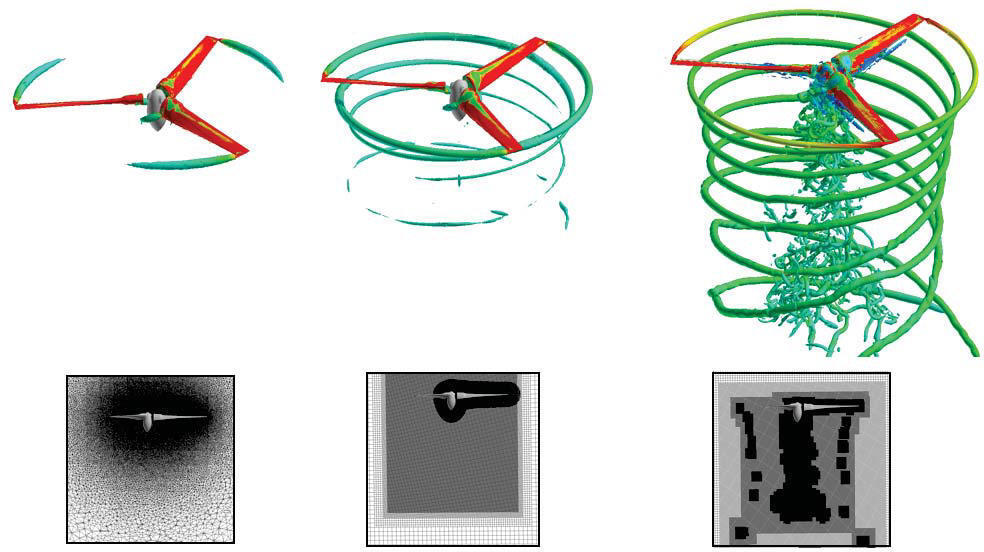
\includegraphics[height=0.3\textheight]{figures/adaptive.jpg}
    \caption{网格自适应加密对涡量分布计算结果的改善\upcite{Sankaran2011}}
\end{figure}

美国斯坦福大学\footnote{Stanford University}的Kamkar和Jameson\upcite{Kamkar2011,Sankaran2011}
提出了一种适用于涡主导流动问题的自适应网格加密方法。
该方法将网格细化过程分为两步:先利用特征检测(Feature Detection)方法自动识别需要加密网格的区域,再利用基于Richardson外插方法的误差估计,给出合适的网格精细程度(分辨率)。
此文所用计算网格为双重网格(dual-mesh),靠近物体表面用非结构网格处理复杂的几何外形及边界层,远离物体表面的区域用自适应结构网格和高阶格式处理涡流尾迹。
基于上述方法,作者计算了机翼翼梢涡和旋翼尾迹等典型的涡主导流动问题。
结果显示,该方法能够同时提高旋翼飞行器性能分析精度和尾迹分辨率。

\subsection{无网格法}
近些年,网格生成技术的发展已落后于数值算法和计算机硬件的发展,日益成为制约计算流体动力学发展和工程应用的瓶颈。
目前,许多网格生成技术的自动化水平较低,网格质量过度依赖研究者的操作经验,并且生成网格需要耗费大量人工劳动时间;
而已有的自动化网格生成方法在处理复杂几何外形时,计算效果并不理想。
解决网格生成问题的一种方案是采用无网格方法。

美国工程院院士Atluri教授\upcite{Atluri1998}
提出了一种基于局部弱形式的无网格方法(Meshless Local Petrov-Galerkin method, MLPG)。
该方法在进行插值和积分时,不再像传统方法(有限差分法、有限元法、边界元法等)那样依赖不重叠的连续网格,因而是一种真正的无网格方法。
该方法已经在固体力学、结构力学、拓扑优化等领域获得了成功应用。

美国加州大学洛杉矶分校\footnote{University of California, Los Angeles}的林洪昌\upcite{Lin2000}
首次将该方法应用到对流扩散输运问题和不可压缩流动问题的分析中。
在求解高$Re$的对流扩散问题时,此文将迎风格式(Upwind scheme)引入到MLPG方法中,解决了解的非物理振荡问题。
在求解不可压缩Navier-Stokes方程时,此文也将迎风格式与MLPG方法相结合,得到了很好的结果。
但此文中的算例比较简单,都是一维、二维问题,对于更加复杂、工程实践中更有意义的三维问题,作者只给出了对于该方法应用前景的乐观预期。
尽管如此,MLPG方法的确解决了网格生成困难这一计算力学领域日益突出的问题,因而有希望在今后得到更广泛的应用。

美国斯坦福大学的Katz和Jameson\upcite{Katz2009}
提出了一种适用于计算流体动力学的无网格方法,并与传统的基于网格的有限体积法进行了对比。
对于二维跨音速、超音速、黏性流动问题(翼型绕流问题),此文提出的无网格算法在计算精度和效率上与大多数有限体积法相当。
此外,把无网格方法应用到重叠网格的无缝连接中,计算结果好于传统的在不同网格之间进行插值的处理方法。
然而, 这里所用的无网格法仍然属于非守恒的算法,因而不能取代基于网格的传统方法。
此文也没有提出具体的计算点生成方法,因而并没有解决传统方法中网格生成难的问题。
Katz认为,无网格法并不会取代传统方法,而只会作为传统的方法在处理一些问题时的补充手段,例如重叠网格的无缝连接问题。
此文只用无网格法求解了二维问题,将其推广到三维问题是该方法未来的发展方向之一。

伊朗阿米尔卡比尔理工大学\footnote{Amirkabir University of Technology}的Sattarzadeh等(2012)\upcite{Sattarzadeh2012}
提出了一种隐式无网格方法,将其用于求解具有复杂几何边界的三维可压缩流动问题,给出了三维机翼、直升机机身绕流等算例,证实了无网格法在流体工程问题分析中的应用潜力。
\begin{figure}[t!]
    \centering
    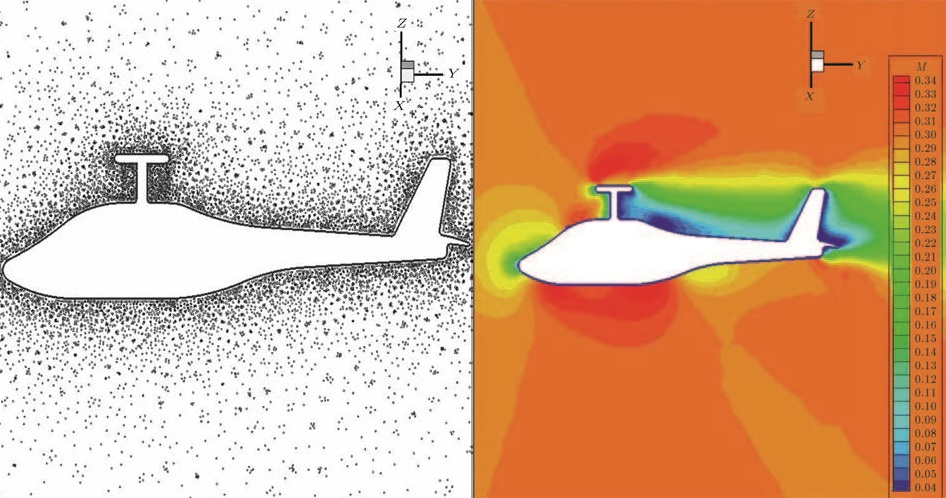
\includegraphics[height=0.3\textheight]{figures/meshless.jpg}
    \caption{由无网格法计算得到的直升机机身表面压力分布\upcite{Sattarzadeh2012}}
\end{figure}

\subsection{其他新方法}

美国斯坦福大学的Jameson教授和Butsuntorn、Allaneau等,在计算流体动力学新方法领域所开展的一些研究,直接或间接地为旋翼空气动力学研究提供了新的工具。

Butsuntorn和Jameson\upcite{Butsuntorn2008}
采用时间谱方法(Time Spectral method)和涡量约束方法(Vorticity Confinement method)研究了旋翼飞行器的流动问题。
时间谱方法在满足工程问题所需精度要求的前提下,显著减少了计算时间,其计算效率大约比传统方法(隐式时间积分格式)提高了10倍。
但是,这种时间谱方法利用了旋翼流场周期变化的特点,因而不适用于机动飞行等非周期工况。
对于结果中含有高频成分的问题,所需计算量将显著增加,从而失去该方法计算效率高的优势。
涡量约束方法较好地模拟了旋翼流场中普遍存在的亚音速和跨音速流动现象。
该方法不需采用传统的网格加密技术,就能使涡结构在较长距离内保持存在。
但是,这种涡量约束方法并没有严格的数学基础。
约束参数的选取与计算精度和稳定性密切相关,但还没有标准的取值方法。
因此,涡量约束方法目前还不是一种成熟的流体动力学计算方法。
另外,此文只研究了刚性、无扭、矩形桨叶在总距和周期变距为常值时孤立旋翼的流动问题,没有考虑桨毂连接形式,也没有考虑机身、尾桨存在时的气动干扰问题。

Allaneau和Jameson\upcite{Allaneau2012}
提出了一种动能守恒非连续Galerkin格式(Kinetic Energy Preserving Discontinous Galerkin scheme, DG-KEP),用于求解Euler方程和低雷诺数的黏性流动问题。
该方法能够保证全局动能守恒,一定程度上解决了数值离散引起的非物理耗散问题,并且大大提高了算法的稳定性。
该方法能够比较真实地模拟机翼尾流的复杂涡结构,从而有助于精确地计算升力和阻力。
在特定情况下,DG-KEP格式成为动能守恒有限体积格式(Kinetic Energy Preserving Finite Volume scheme, FV-KEP)。
这是一种特殊的中心格式,比常规的通量平均中心格式更加稳定,且不需引入人工耗散。
对于黏性流动问题,适当选取网格雷诺数几乎可以完全消除数值解的非物理振荡,并且计算成本远低于引入人工耗散的常规中心格式。
在二维激波管算例中,该格式成功捕捉了激波和声波,验证了算法的有效性。
在此基础上,研究了激波与涡的相互干扰,对非定常运动的二维翼型进行了直接数值模拟,对三维可变形机翼也进行了流固耦合分析。
该算法在这些简单算例中所表现出了低数值耗散的特点,有助于解决传统CFD方法在计算桨尖涡时存在非物理耗散的弊端,但目前还没有被直接应用到直升机或旋翼空气动力学的研究中。

%\subsection{并行计算}

%%%%%%%%%%%%%%%%%%%%%%%%%%%%%%%%%%%%%%%%%%%%%%
\section{舰载直升机舰面空气动力学}
舰载直升机所特有的空气动力学问题,主要表现为海面自由来流和舰船空气尾流与旋翼尾迹的相互作用。
起飞和着陆过程中,海面和舰面阻挡旋翼尾迹向下游移动,引起的“地”面效应,也是影响直升机飞行安全的重要因素。
研究海面、舰面与旋翼之间的气动干扰,是舰载直升机舰面空气动力学的主要任务。
与旋翼空气动力学类似,该领域的研究方法也分为实验和计算两大类。

\subsection{实验研究}
美国航空航天计算公司\footnote{Aerospace Computing, Inc.}的Derby和美国国家航空航天局\footnote{National Aeronautics and Space Administration, NASA}Ames研究中心的Yamauchi\upcite{Derby2003}
介绍了一套用于研究旋翼飞行器与两栖攻击舰气动干扰问题的$1/48$缩比模型方案。
该尺寸的选择主要是为了能够在NASA Ames研究中心的$7\times10~\mathrm{ft}$风洞中开展吹风实验。
另外,该模型还被用于研究旋翼飞行器与大型建筑物以及地面的气动干扰问题。
该项目对倾转旋翼机、纵列式直升机、单主旋翼直升机三种构型都进行了缩比模型实验。
获得的结果可用于指导全尺寸直升机舰上操纵以及编队飞行的研究。

美国NASA Langley研究中心的Lamar等\upcite{Lamar2004,Lamar2007}
通过实验研究了利用柱状涡流发生器(Columnar Vortex Generator, CVG)对船体空气尾流进行控制的可行性。
作者希望该技术能够应用于改善舰载机(包括直升机)的起降环境。
\begin{figure}[t!]
    \centering
    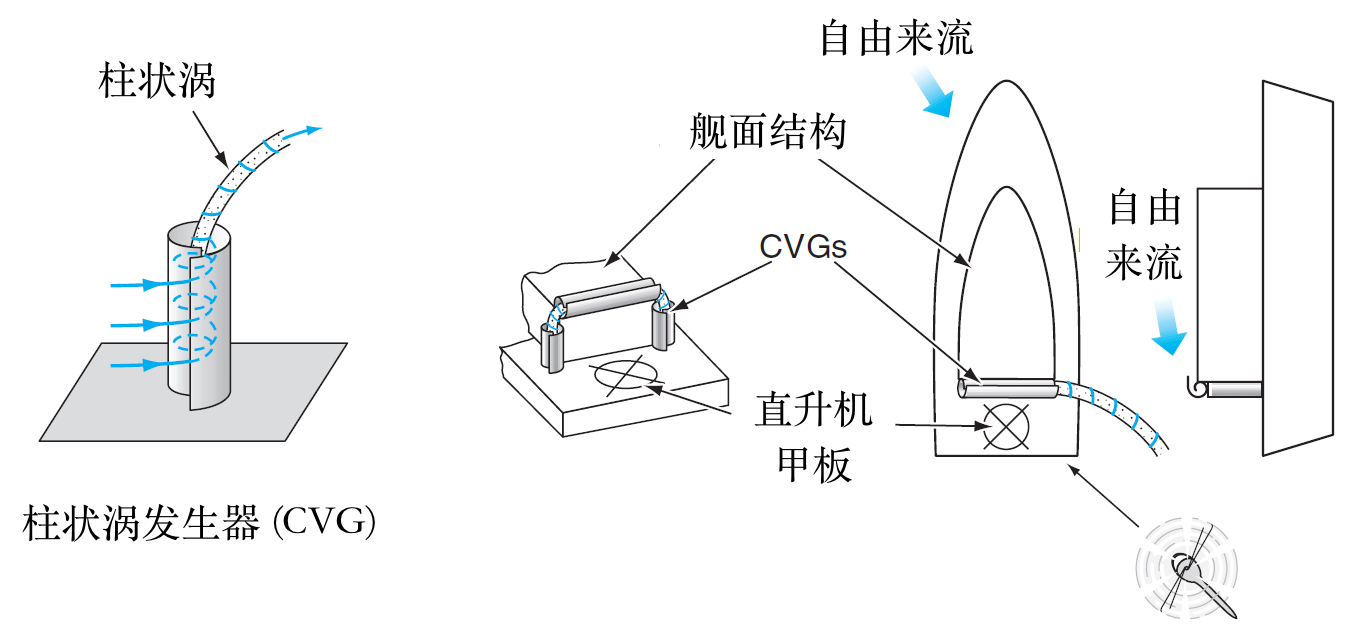
\includegraphics[height=0.3\textheight]{figures/modifying.png}
    \caption{利用柱状涡流发生器改善舰载直升机起降环境\upcite{Lamar2004}}
\end{figure}

法国航空航天研究中心\footnote{Office National d'Etudes et de Recherches Aerospatiales, ONERA}的Herry
和荷兰国家航空航天实验室\footnote{National Aerospace Laboratory}的Vorst\upcite{Herry2011},
利用粒子成像测速技术和激光断层扫描显示(Laser Tomoscopy Visualizations, LTV)技术,
在ONERA的L2风洞中测量了$1/60$简单外形军舰缩比模型和$1/100$真实外形军舰缩比模型两种船体的空气尾流。
实验结果对于理解船体无侧滑航行时,船体结构后方气流的双稳定(bi-stable)现象,特别是二者之间的临界情况有很大帮助。

英国利物浦大学\footnote{University of Liverpool}的Kääriä等
与澳大利亚棱镜防务公司\footnote{Prism Defence Pty. Ltd.}的Forrest
以及英国林肯大学\footnote{University of Lincoln}的Owen\upcite{Kaeaeriae2012}
通过开展水洞实验,研究了直升机处于舰体空气尾流中时的气动载荷特征。
该实验是在一个$1/54$的直升机缩比模型上进行的,模型直升机的旋翼也进行了简化,气动载荷通过安装在机身内的六分量天平来测量。
实验模拟了船头正面迎风与$45~\deg$侧风两种来流条件,沿直升机着舰机动飞行路径选取了几个固定点,测量了直升机在这几个点上的非定常气动载荷。
结果表明,船头正面迎风时,直升机着舰过程中存在“拉力不足”(thrust-deficit)的区域;
而在$45~\deg$侧风条件下,存在“压力墙”(pressure-wall)区域。
作者认为,这是由船体空气尾流中的速度梯度引起的,通过对船体空气尾流进行非定常CFD分析,解释了上述实验观察到的现象。
尽管该实验是在固定直升机的条件下进行的,仍不能完全反映直升机着舰过程的真实载荷特征,但可作为验证计算模型的参照对象。

美国乔治华盛顿大学\footnote{The George Washington University}的Friedman和Snyder,
以及法国空军学院\footnote{French Air Force Academy}的Duplessis\upcite{Friedman2015}
利用固定在(长$32.9~\mathrm{m}$)实验船后甲板上的模型直升机,研究了船体空气尾流与直升机旋翼尾迹的相互影响。
通过安置在旋翼周围的风速计,测量了实验船静止、无侧风航行、侧风航行等条件下的流场信息。
尽管该实验是在固定直升机的条件下进行的,但已将实验环境从室内转移到了真实的船只上,因而更接近舰载直升机的真实工作环境。

\subsection{数值计算}
美国海军研究实验室\footnote{Naval Research Laboratory}的Landsberg等\upcite{Landsberg1995}
利用FAST3D非定常流动求解器,分析了船体空气尾流与旋翼入流的相互作用。
FAST3D求解器采用的是通量修正输运(Flux Corrected Transport, FCT)算法和虚拟单元嵌入(Virtual Cell Embedding, VCE)方法。
旋翼对流场的影响是通过一个简化的下洗模型(即动量源模型)来体现的,该模型中动量通量沿桨盘平面均匀分布,因此只能反映旋翼整体的气动特性,而不能精细到到每片桨叶。
虽然计算模型较为简单,但计算结果仍能反映船体空气尾流中的非定常性对旋翼入流的影响。

荷兰国家航空航天实验室的Muijden等\upcite{Muijden2013}
基于结构网格,求解RANS方程和RANS-LES混合方法两种物理模型,分析了船体空气尾流,并与实验数据进行了比较。
结果表明,RANS方程的计算结果很好地反映了船体空气尾流的时间平均特征,而RANS-LES混合方法则进一步给出了更加接近物理真实的流场波动特征。
上述计算结果已被用到直升机飞行模拟器中,并且得到了经验丰富的飞行员给出的积极评价。
但此文只计算了船体空气尾流,并没有将直升机(特别是旋翼)包括在计算模型中,因此没有体现船体空气尾流与旋翼空气尾流的耦合效应。

英国利物浦大学的Crozon等\upcite{Crozon2014}
基于结构网格,利用作用盘方法对旋翼在船体影响下的入流特征进行了静态计算。
作用盘方法的结果表明,当旋翼接近船体时,其入流会受到船体的显著影响,这种影响是非线性的,因而叠加法不再适用。
为突破作用盘方法只能描述旋翼整体入流特征的限制,作者通过求解非定常RANS方程获得了每片桨叶的流场信息。
通过该方法得到的旋翼拉力的计算结果与实验结果吻合较好,验证了方法的有效性。
作者希望此文的计算方法有助于确定直升机着舰过程的安全飞行包线,但并没有给出具体的结论。
就算例而言,此文也只给出了孤立旋翼与船体在气动方面的相互影响,没有考虑机身对气流的影响,也没有考虑旋翼动力学方面的问题。

美国先进旋翼机技术公司的He等\upcite{He2008}
介绍了该公司在建立高置信度舰载直升机飞行仿真环境方面所做的工作。
该仿真系统集成了直升机动力学、船体动力学以及非定常船体空气尾流方面的建模方法,为舰载直升机飞行训练和测试提供了一种高效的模拟工具。
该仿真系统提供了三种不同精细程度的仿真模型:
\begin{compactitem}
  \item 旋翼尾迹由有限状态入流模型描述,船体空气尾流由平板模型描述;
  \item 旋翼尾迹由有限状态入流模型描述,船体空气尾流由CFD或实验数据描述;
  \item 旋翼尾迹和船体空气尾流由黏性涡粒子方法描述。
\end{compactitem}
其中,前两种模型可用于实时仿真计算。

此后,该公司的Zhao等\upcite{Zhao2013}
采用一种基于物理学原理(Physics-Based)的建模方法,对旋翼飞行器与船体的气动干扰问题进行了研究,并在此基础上进行实时飞行仿真研究。
作者将黏性涡粒子方法(VPM)与基于非结构网格的CFD求解器相结合,研究了旋翼尾迹与船体空气尾流之间复杂的相互作用关系。
基于VPM/CFD混合方法的计算结果,作者对Peters-He有限状态入流模型进行了推广,使其适用于实时仿真。

\section{舰载直升机相关应用问题简介}
除了空气动力学以外,舰载直升机的应用还面临许多舰面动力学、飞行动力学、导航和飞行控制等方面的问题。

\subsection{舰面动力学}
美国卡曼航空航天公司\footnote{Kaman Aerospace Corporation}的Wei等\upcite{Wei1992}
分析了SH-2F型直升机在预定的甲板运动、甲板摩擦、定常风条件下的舰面动力学特性,用以确定该型直升机安全着舰和离舰的条件。
对处于工作状态的旋翼、处于非工作状态的旋翼、折叠起来的旋翼以及机身分别进行了建模,以研究这四种情况的空气动力学特性。
利用能量法推导了船体运动的动力学方程,包含三个线位移、两个角位移(滚转、俯仰)共五个自由度。
此外,作者还分析了不同甲板摩擦条件对直升机舰面动力学特性的影响。
基于上述分析模型,此文给出了一些定性和定量的安全指标,但有待实验数据的验证。

加拿大卡尔顿大学\footnote{Carleton University}的Wall\upcite{Wall2009}
研究了舰载直升机着舰和离舰过程中桨叶特有的气弹问题。
在海上风速较大且旋翼转速较低时,桨叶容易出现较大变形,这是由桨叶的动力学特性、船体运动、船体空气尾流等因素共同作用所引起的。
作者将柔性桨叶离散为若干刚性的微段,用以表现非线性的桨叶弯曲变形;
基于实验数据对船体空气尾流进行建模,体现了甲板上方气流随时间、空间变化的非定常、非均匀的特征。
此文反映了影响桨叶气弹响应的各种因素之间相互作用关系的复杂性,但分析所用气动模型依赖实验数据,可考虑用更一般的CFD方法代替。

\subsection{飞行动力学}

美国NASA Ames研究中心的Paulk Jr.等\upcite{PaulkJr1983}
通过仿真研究发现,紊乱的舰面气流是影响直升机着舰飞行最关键的环境因素。
为保证飞行性能,需采用高度指令补偿系统。

美国系统技术公司\footnote{Systems Technology, Inc.}的Jewell等\upcite{Jewell1986}
介绍了一项由美国海军航空发展中心\footnote{Naval Air Development Center}支持的实验研究。
该项研究的目的是在直升机操稳参数、舰面操纵流程、环境条件等方面,对飞行品质规范修订提出建议。

此后,该公司的Clement等\upcite{Clement1992}
建立了一种用于模拟直升机着舰飞行的实时仿真模型。
该模型采用叶素法对旋翼进行气动建模;
利用CFD软件得到船体空气尾流数据,并经过三维FFT算法处理,使其适用于实时仿真。

美国佐治亚理工学院的Zhang等\upcite{Zhang1994}
利用全尺寸海上实验数据,识别出一个关于船体空气尾流速度垂直分量的功率谱模型。
基于上述半经验的船体空气尾流模型和一个简化的旋翼气动模型,作者研究了船体空气尾流对旋翼拉力和滚转、俯仰力矩的影响。
此后,作者又建立了一种用于模拟直升机与船体气动干扰并考虑地面效应的实时仿真模型。
该模型中,船体由板块表示,旋翼尾迹由固定尾迹和预定尾迹模型表示,海面的影响(地面效应)通过镜像法体现。
基于以上模型,将旋翼入流表示成有限状态形式,以便于进行实时仿真。
该模型只适用于直升机在甲板上方悬停的配平问题。
此后,作者还直升机与船体气动干扰问题中的地面效应问题进行了研究\upcite{Zhang1995}。

加拿大NTI公司\footnote{Newmerical Technologies International Inc.}的Bogstad等
以及CAE电子公司\footnote{CAE Electronics Ltd.}的Giannias等\upcite{Bogstad1999,Bogstad2002}
利用有限元求解器,基于Euler方程和非结构网格技术,研究了船体空气尾流,并将得到的数据整合到直升机飞行仿真软件中。
加拿大国家研究委员会\footnote{National Research Council of Canada}的Zan\upcite{Zan2003}对\cite{Bogstad2002}中的一些观点提出了质疑。
Zan认为,特殊算例的CFD计算结果与实验数据进行的对比,并不能证明该CFD方法在更一般的条件下下仍然有效。
实验和基于Navier-Stokes方程的计算结果都显示,在某些情况下,船体空气尾流是由涡流主导的,并且存在强烈的流动分离现象。
因此,\cite{Bogstad2002}中基于Euler方程得到的结论并不可靠。

美国宾夕法尼亚州立大学\footnote{Pennsylvania State University}的Lee等\upcite{Lee2003,Lee2005}
基于非结构网格,利用定常和时间精确(非定常)无黏CFD计算得到船体空气尾流,并将其引入到GENHEL直升机飞行仿真程序中。
基于此模型,作者针对特定的直升机着舰和离舰飞行轨迹,设计了最优控制算法。
结果表明,船体空气尾流的非定常性对于直升机着舰和离舰操纵具有显著影响,这正是舰载直升机与舰载固定翼飞机明细不同的地方。
此文中的CFD计算模型没有考虑空气黏性,因而可能没有丢失了一些真实船体空气尾流的特征。
在\cite{Lee2004}中,Lee等引入了一种随机船体空气尾流模型 ,用以提高仿真的效率。
该模型可用于优化飞行控制系统,以提高飞行器抗扰性能。

荷兰代尔夫特理工大学\footnote{Delft University of Technology}的Hoydonck等\upcite{Hoydonck2006}
建立了一种用于模拟直升机着舰操纵的飞行力学模型。
旋翼模型采用刚性桨叶,考虑二阶挥舞运动,用叶素法对主旋翼进行建模。
旋翼入流采用一种改进的Pitt-Peters动态入流模型进行建模,通过引入四个状态变量来体现尾迹畸变对旋翼入流的影响。
利用该模型,作者研究了直升机按预定路径着舰的飞行稳定性和控制方面的一些问题,但并没有考虑船体空气尾流对旋翼的影响。

澳大利亚棱镜防务公司的Forrest,英国林肯大学的Owen,英国利物浦大学的Padfield以及英国BAE系统公司\footnote{BAE Systems}的Hodge\upcite{Forrest2012}
将非定常CFD计算所得的船体空气尾流数据引入到直升机飞行模拟器中,得到了一个比较接近真实情况的飞行仿真环境。
一些直升机着舰飞行过程中真实存在的现象,在该仿真模型中得到了体现。
通过飞行员的主观评价以及其他客观指标,验证了该模型的有效性,也验证了将船体空气尾流CFD计算结果引入飞行仿真的可行性。
尽管该方法只考虑了船体空气尾流对旋翼尾迹的影响,但仍可应用于舰载直升机飞行员的日常训练。

美国弗吉尼亚理工学院\footnote{Virginia Polytechnic Institute and State University}的Ngo和Sultan\upcite{Ngo2014}
建立了一种用于着舰操纵的面向控制系统设计的非线性直升机飞行力学模型。
该非线性模型具有隐式常微分方程的形式,其结果与基于悬停和前飞状态线化模型的结果吻合较好。
此外,作者用一种简单的船体运动模型来模拟海面不规则运动对船体的影响。
基于以上直升机模型和船体模型,作者利用模型预测控制(Model predictive control, MPC)方法,设计了一种能够完成自主着舰任务的控制系统。
从工程实践角度看,该模型具有一定的应用价值,但该模型所用的Pitt-Peters静态入流模型,并不能体现旋翼与船体在气动方面的相互影响。

美国联合学院和大学\footnote{Union Institute and University}的Akinyanju\upcite{Akinyanju2007}
基于FLIGHTLAB旋翼飞行器综合分析软件,对舰载直升机舰面操纵进行了建模和分析,并将仿真结果与实验数据进行了比较。
作者采用叶素法、有限状态尾迹和自由尾迹对旋翼进行建模,基于CFD对船体空气尾流进行模拟,引入地面涡(Ground Vortex)模拟甲板和海面引起的地面效应。
计算结果表明,船的航行速度、航向、旋翼转速、海况对直升机的舰面操纵具有显著影响,并且得到了实验数据的验证。
但此文中的建模工作过于依赖软件提供的功能,因而不具有一般性,也不易引入更精细的气动或动力学模型。

\subsection{导航与飞行控制}

美国Lear Siegler公司\footnote{Lear Siegler, Inc.}的Gevaert等\upcite{Gevaert1978}
提出了一种全自动直升机舰面回收系统的设计方案。
针对高海况条件下的舰载机着陆任务,设计了导航和控制系统算法。
作者将六自由度直升机飞行动力学模型和船体运动数据用于全自动和远程人在回路仿真。

以色列理工学院\footnote{Israel Institute of Technology}的Negrin等\upcite{Negrin1991}
介绍了一种用于手动执行直升机在移动甲板上方低空悬停任务的叠加显示技术。
分析和实验结果表明,将惯性参考系中的位置信息提供给飞行员,有助于提高直升机在移动甲板上方执行悬停任务的质量。

美国加州大学戴维斯分校\footnote{University of California, Davis}的Hess\upcite{Hess2005}
基于简化的船体运动和直升机飞行动力学模型,提出了一种适用于旋翼飞行器全包线飞行控制系统设计的方法,并将该方法应用于直升机在高速航行的舰船甲板附近执行位置保持任务。

\chapter{结论}
随着我国海洋强国战略的逐步实施,我国在海上的军事、科考和生产活动正变得日益频繁。
与之相伴的是海上作业任务的不断丰富,以及对舰船海上作业半径和反应时间要求的不断提高。
飞行器以其远高于舰船的运动速度,能够极大地延伸舰船作业半径,缩短反应时间。
固定翼飞机对起降平台的要求较高,通常只有在具有数百米长跑道的航母上才能完成。
直升机以其特有的垂直起降能力,可以在与其尺度大致相当的平台上完成起降,因而比固定翼飞机更广泛地应用于海上作业。

但是,海面复杂多变的气流和海浪条件,船体对海面气流的非定常扰动,海面、船体与旋翼之间的气动干扰,
使得直升机在舰面完成起降任务的难度远大于其在陆地上执行起降任务,也大于固定翼飞机在航母平台上执行舰面起降任务。
着舰和离舰是舰载直升机执行任何海上作业任务都必须完成的飞行科目。
为确保舰载直升机安全完成舰面起降任务、减轻飞行员工作负担,有必要对舰载直升机的空气动力学、舰面动力学、飞行动力学、导航和飞行控制方法开展深入研究。
其中,空气动力学是后续几项研究内容的基础。
本文对舰载直升机空气动力学的国内外研究现状进行了综述,并对与舰载直升机相关的一些应用问题作了简要介绍。

舰载直升机空气动力学研究,既包含所有旋翼飞行器共有的一般性问题(即通常意义下,旋翼空气动力学所包含的研究内容),也有海面和船体与旋翼相互影响所带来的特殊问题。
旋翼空气动力学研究的主要任务是,认识旋翼流场的特点和规律,为旋翼飞行器的设计、使用和维护提供支持。
舰载直升机舰面空气动力学研究的主要任务则是,深入理解旋翼尾迹和船体空气尾流的流动特点,
把握海面、船体与旋翼之间的气动干扰规律,为舰载直升机舰面动力学、飞行动力学、导航和飞行控制方法研究提供支持。
这两大类问题的研究方法均可分为实验和计算两类。

对旋翼空气动力学的实验研究经历了从定性到定量,从宏观到微观的发展过程。
最开始,人们通过自然凝结现象,观察到了旋翼桨尖涡的存在,并认识到旋翼流场由桨尖涡主导的重要事实。
此后,喷烟法、阴影法、纹影法等流动显示方法不断被引入旋翼空气动力学的定性实验研究中。
定量实验方面,包含测力实验和测速实验两类。
伴随实验技术的进步,测速实验经历了侵入式热线测速技术、非侵入式单点LDV技术、非侵入式多点PIV技术的发展过程。
目前,三维PIV技术已经能够对旋翼流场进行高分辨率测量,可以预见,该技术在未来一段时间里仍将是旋翼空气动力学研究的重要工具。

数值计算是旋翼空气动力学的另一类重要的研究方法。
旋翼流场的非定常、非线性特征决定了问题的复杂性。
为了真实还原旋翼流场的流动特征,必须解决好转捩、附面层分离、涡核粘性耗散、涡结构失稳破裂等复杂的流体力学问题。
在连续介质力学框架内,只有直接数值模拟技术可以完全实现上述目标。
受限于计算机硬件和软件发展水平,将DNS技术直接应用到旋翼空气动力学计算上,目前看来还很不现实。
因此,有必要寻找切实可行的替代方法。
旋翼入流模型、涡线尾迹模型、黏性涡粒子模型、基于欧拉观点的涡量输运模型、雷诺平均Navier-Stokes方程模型等,都已经被直升机工程界所采用。
为了解决网格离散带来的涡量非物理耗散问题,网格自适应加密技术、涡量约束方法等新兴的流体力学计算方法正成为该领域的研究热点。
而无网格法以其处理复杂几何边界的灵活性,也逐渐引起了计算流体力学界的关注。

除上述旋翼空气动力学的一般性问题外,舰载直升机还有一些海上作业、舰面起降所带来的特殊空气动力学问题。
这类特殊问题主要表现为海面自由来流、舰船空气尾流与旋翼尾迹的相互作用,即气动干扰问题。
美国、法国、荷兰等国在该领域开展了许多实验和计算方法研究,一些分析方法已经实现商业化,并成功应用到飞行仿真、导航和飞行控制系统设计等应用领域。
相比之下,我国在这方面开展的研究工作十分有限。
研究舰载直升机空气动力学,特别是海面、舰船与旋翼之间的复杂气动干扰问题,
对于确定直升机舰面起降的环境条件,制定和完善直升机舰面起降作业规程,提高舰载直升机的安全性和作业效率具有重要意义。

% 参考文献
\cleardoublepage
\phantomsection
\addcontentsline{toc}{chapter}{参考文献}
\bibliography{reference}
\cleardoublepage

\end{document}
